\documentclass[english,11pt,a4paper]{article}
\usepackage[utf8]{inputenc}
\usepackage{mathtools}	%
\usepackage{amssymb} % Mathematik und Dinge wie \qquad
\usepackage[T1]{fontenc} %Anführungszeichen
\usepackage{graphicx} %Bilder
\graphicspath{/Users/Nata/Documents/Master/M Prak Biophysics/Genetic Toogle Switch}
\usepackage{subcaption} %figures nebeneinander
\usepackage[labelformat=simple]{caption} %Bildunterschriften
\usepackage{setspace}
\usepackage{nicefrac}
\usepackage{longtable}
\usepackage[english]{babel}
\usepackage{array}
\usepackage{float}
\usepackage{geometry}
\usepackage{physics}
\usepackage[colorlinks=false]{hyperref}
\usepackage[miktex, subfolder]{gnuplottex}
%\usepackage[parfill]{parskip} % Absätze nicht eingerückt sondern durch Leere Zeilen getrennt
\setlength\parindent{0pt}
%
\usepackage{biblatex}
\usepackage{filecontents}
\usepackage{bibgerm}
\usepackage{url}

\usepackage{chemmacros,upgreek} 
\NewChemParticle\neutrino{\chemnu_{$\!e$}} 
\NewChemParticle\antineutrino{$\bar{\chemnu}$_{$\!e$}} 

\NewChemParticle\betaminus{\chembeta-} 
\NewChemParticle\betaplus{\chembeta+}


\begin{filecontents}{quellen.bib}	
{
	@online{1,
		title = {Manual},
		url = {http://apcmbp.uni-koeln.de/sites/biophyspraktikum/Prelab_Manual_FRET.pdf},
		urldate = {2017-12-02},
	}
	@online{2,
		title = {Refractive index of water},
		url = {http://hyperphysics.phy-astr.gsu.edu/hbase/Tables/indrf.html},
		urldate = {2017-12-02},
	}
	@online{3,
		title = {Quantum yield of Cy3},
		url = {http://www.atdbio.com/content/32/Cyanine-dyes},
		urldate = {2017-12-02},
	}
	@online{4,
		title = {Extinction coefficient of Cy5},
		url = {http://www.sigmaaldrich.com/technical-documents/protocols/biology/sample-labeling-and-processing.html},
		urldate = {2017-12-02},
	}
	@online{5,
		title = {Fluorescence spectroscopy},
		url = {https://de.wikipedia.org/wiki/Fluoreszenzspektroskopie},
		urldate = {2017-12-02},
	}

	@online{6,
		title = {Förster Radius of Cy3-Cy5},
		url = {https://web.stanford.edu/class/cs379c/archive/2013/class_messages_listing/figures/fluorescence_resonance_energy_transfer.pdf},
		urldate = {2018-01-12},
	}
}
\end{filecontents}
\addbibresource{quellen.bib}

\linespread{1.4}

%================================================================================

\begin{document}

\begin{titlepage}
	\centering
	\huge
	\textbf{Genetic toggle switch}
	
	\vspace{1cm}
	\huge
	Advanced Practical course in Biophysics
	
	\vspace{0.8cm}
	\normalsize
	at the
	
	\vspace{0.5cm}
	\Large
	Institute for Theoretical Physics, \\ University of Cologne
	
	\vspace{1cm}
	\normalsize
	April 17, 2018
	
	\vspace{1.5cm}
	\begin{figure}[h]
		\centering
	%	\includegraphics[width=150pt]{resources/uni_logo.png}
	\end{figure}
	
	\vspace{2.5cm}
	\small
	
	\begin{centering}
		\begin{tabular}{lll}
			& \textbf{Students} & \hspace{5cm} \textbf{Instructor} \\
			& Simon Barton 5963508 & \hspace{5cm} Martin Lukacisin \\
			& Galib Hassan 6057349\\
			& Natawan Gadjisade 6045910
		\end{tabular}
	\end{centering}
	
\end{titlepage}

\pagenumbering{Roman}  
\tableofcontents

\pagebreak
\pagenumbering{arabic}

\addcontentsline{toc}{section}{Introduction}
\section*{Introduction}

A genetic toggle switch has a similar function as a flip flop in electronics.
In a genetic circuits the genetic toggle switch can exhibits two stable steady states and store 1 bit of information.
In this experiment we are observing the behaviour of a genetic toggle switch as well as its switching between two stable states (two different fluorescent proteins with different colours, green and red) bacteria E.Coli is observed..
As the E.coli bacteria are genetic modified with two different promoters which not only control the expression of two genes but also the expression of a repressor for each other, the system is in a steady state of the circuit.   
Measuring the fluorescence of the system allows us  to determine the concentration of the inducer that is needed to cause a switching between the green and red fluorescent protein.

\newpage
\part{Theoretical background}

\section{Synthetically controlling gene expression}

The idea behind synthetic gene regularity circuits such as toggle switch is that the transcription of the gene is controlled by inducible promoters by changing the external concentration of an inducer.
It is a easy way to turn genes on and off and to control their level of expression.
The most used inducible promoters are the lac promoter and the tet promoter. 
The transcription factors (such as lac repressor lacl and the tet repressor TetR, respectively) bind to the promoter and repress the transcription of the promoter. 
These repressors can bind to specific inducers as IPTG or aTc. 
The change in protein conformation followed from a change in affinity for the binding site in the promoter region is achieved by the binding of the inducers to the repressors.
The advantage of IPTG and aTc is that they do not have other effect on the cell beside of changing the binding affinity of the respective repressors.

In this experiment the inducible promoters control a reporter gene (e.g fluorescent protein such GFP) and are put on the chromosome or on a plasmid inside a bacterium like E.Coli. 
In growth medium these bacteria are then cultured that can be supplemented with the respective inducer.

\begin{figure}[htbp] 
  \centering
     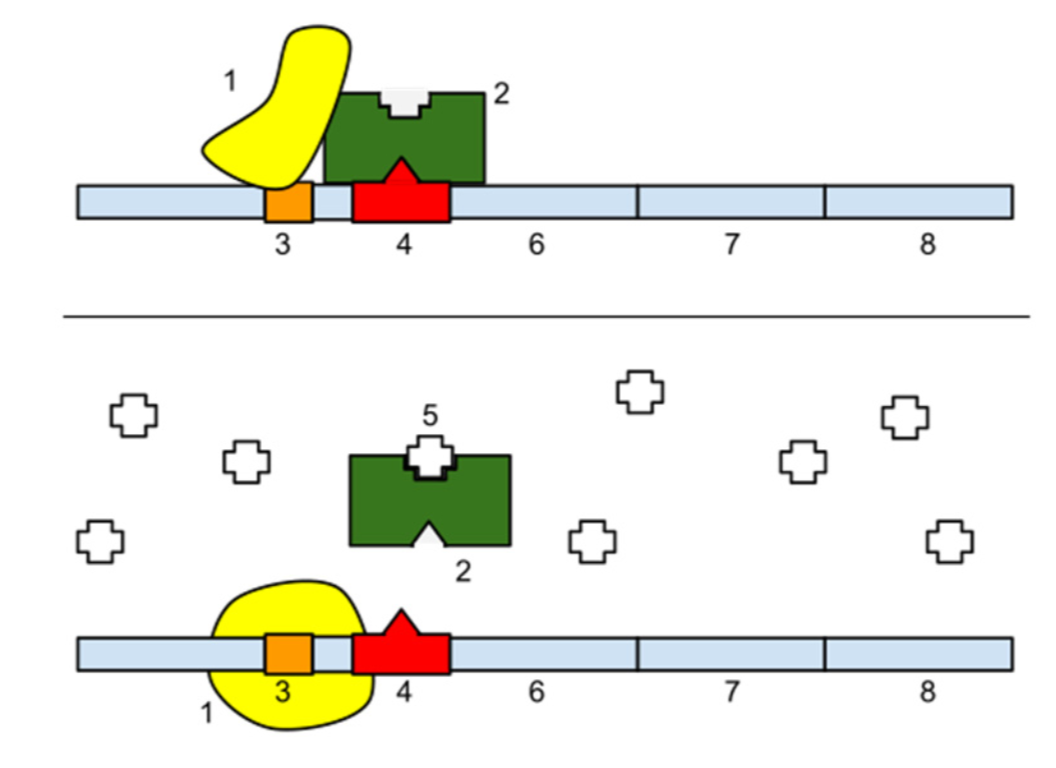
\includegraphics[width=0.7\textwidth]{IPTG}
  \caption{Inducible control of the lac promoter using IPTG. 1: RNA polymerase, 2:Repressor, 3:Promoter, Operator, 5: Lactose, 6-8: lac operon or other genes under the control of the lac promotor. 
 First scheme: The promoter is turned off. No lactose or IPTG is there to block the lac repressor, so the repressor and promoter are tightly bound to the operator, which obstructs the RNA polymerase from binding to the promoter.
Second scheme: The promoter is turned on. Lactose inhibits the repressor, allowing RNA polymerase to bind the promoter and express the downstream genes. Source: Manual of practical course. }
  \label{fig:Bild1}
\end{figure}



\newpage

\section{Design of toggle switch circuit} 

The goal is to obtain two district states of gene expression that are stable over a long. 
This construction consists of two promoters. Each is controlling the the expression of the repressor of the other promoter. 
It allows us to have to possible states. (a) Promoter 2 is shut down as promoter 1 is highly expressed, which leads to many copies of repressor 2.
(b) Promoter 1 is shut down as the promoter 2 is highly expressed, which leads to many copies of repressor 1.

More precisely, here the lac promoter (repressed by Lacl) controls the expression of tetR while the tet promoter (repressed by TetR) controls the expression of lacl. Also the expression of a gfp gene and an mcherry gene is controlled from tet promoter and lac promoter, respectively. 
It is possible to read out the state of the system by measuring fluorescence as gfp code for green and mcherry for red fluorescent proteins (GFP and RFP).
Adding the inducers IPTG or aTc leads to a flipping of the system.


\begin{figure}[htbp] 
  \centering
     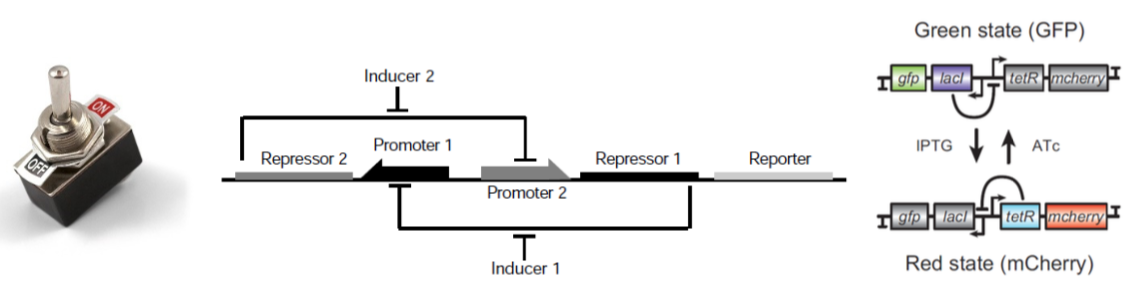
\includegraphics[width=0.9\textwidth]{Design}
  \caption{ Genetic toggle switch. First: electrical toggle switch with a mechanical lever. Second: General design of a genetic toggle switch. Third: Specific circuit used in this experiment (Lee et al.2016). IPTG and aTc can be used to flip the toggle switch from the green to the red state and vice versa, respectively. Source: Manual of practical course }
  \label{fig:Bild2}
\end{figure}

\newpage
\section{Experimental techniques and procedure}

We want to determine the average state of the synthetic toggle switch circuit in a population of cells. For that we have to measure the intracellular concentration of the green and the red fluorescent protein. 
The simplest way is to measure the total fluorescence intensity and normalising it to the total biomass of the population. 
We are using an \textbf{optical density (OD)} measurement to get the biomass of a growing bacterial culture as it is approximately equal to the total cell volume.
The absorbance is measured in a spectrophotometer according to Beer-Lambert law, which is proportional to the biomass density of the culture. Furthermore, measuring the optical density over time allows to determine the specific growth rate.
\\
The individual cells should be after switching either in one of two distinct gene expression states. Here: green or red. 
To observe the single-cell fluorescence we are using a \textbf{fluorescence microscopy} where individual cells are directly visualised.
\bigskip



\section{Set up}
We started our experiment with 4 wells containing 2mM IPTG and 4 wells containing 100 ng/ml aTc with glucose M9 and chloramphenicol. We then added another set of 8 wells containing the same content but making the amount half to the previous set. We repeated the process several times and thus achieve a concentration gradient of IPTG and aTc shown in figure (\ref{concGrad}). 

We also had two overnight cultures (ONC1 and ONC2) of \textit{E. Coli} bacteria where ONC1 and ONC2 were in \textit{green} and \textit{red} states respectively, and also with a wild type MG1655 bacteria. We inoculated the IPTG and aTc wells with these bacteria. 

We took measurement of the optical density from the GFP and RFP fluorescence every $\approx$ 30min. and simultaneously took images with the microscope of the overnight cultures. Furthermore, pictures of the GRP and RFP intensities of overnight cultures mixed with IPTG and aTc, respectively in the highest concentration were also taken.


 
\newpage
\part{Results}





\section{Optical density and growth rate measurement}
The data that was achieved from the experiment provided us with the optical density (OD)of the cultures showed in figure (\ref{concGrad}. All the evaluation has been done using Mathematica and MATLAB software. We have reserved all the relevant codes in a github repository [2]. 

We measured the OD of each cell over time to observe if it shows the exponential nature of the bacterial growth rate. Since linearity in the logarithm scale is equivalent to the  exponentiality in the usual scale, we generated a logarithmic plot against time for each well. Figure (\ref{ODLogPlot}) shows these plots in detail.

OD can be treated as a good measure of bacterial growth rate since it increases with the number of bacteria. We subtracted the OD containing no bacteria from OD's of all cultures and generated the plots1. 

It is noticeable that the concentration of IPTG in A1-B8 and E1-F8 wells did not affect the growth rate much. This is desirable because we put the wild type MG1655 bacteria there, which can grow irrespective of the supplied media. 

C1-D8 and G1-H8 wells, where we mixed the ONC1 and ONC2 bacteria respectively show a similar exponential growthrate at least up to 10000 seconds from the experiment started. However, we expected to see stiffer curves in the right portion of of the plot-grid and flatter in the left portion which would signify the concentration gradient of the medium. From our data, it is not very clear if the concentration gradient affected the growth-rate significantly. 



We applied a linear fit on each of these data-sets and quantified the growth-rate as the slope of the linear fit. 

\begin{figure}[htbp]
\centering
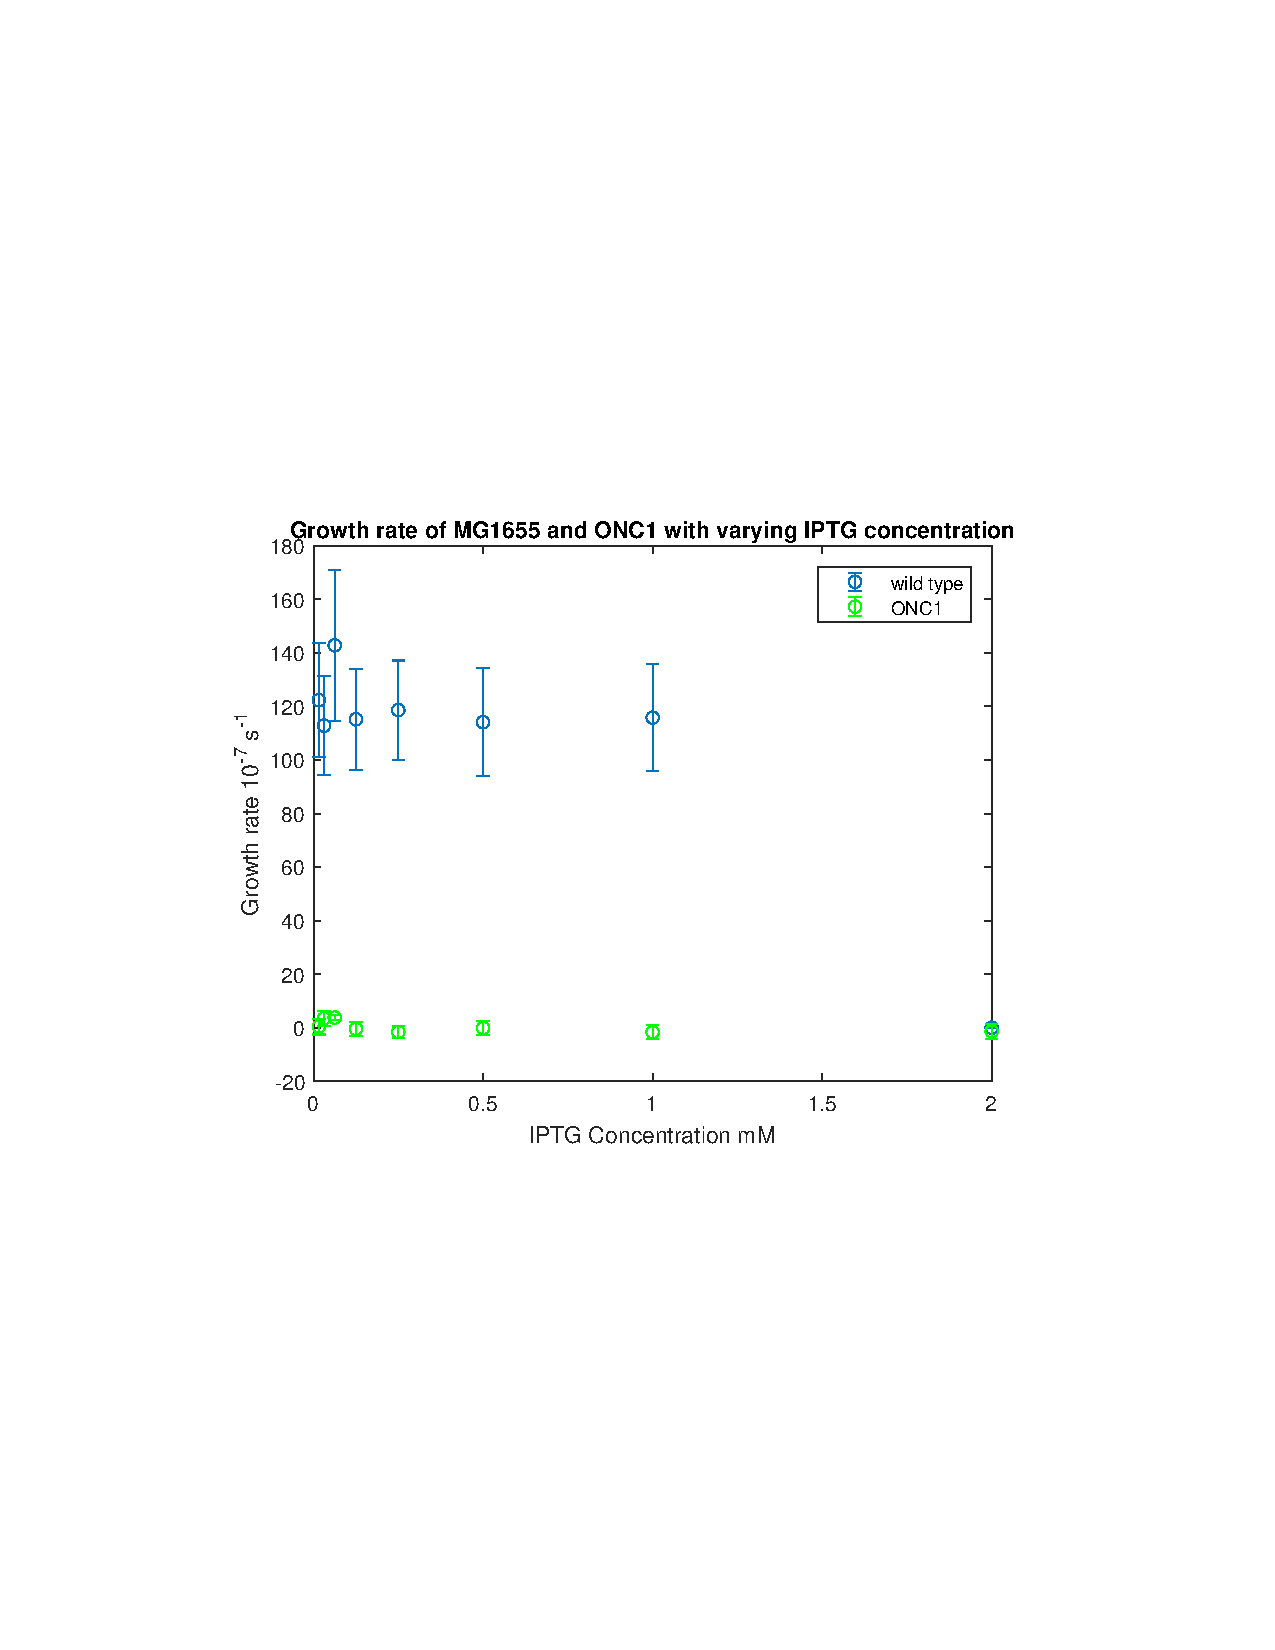
\includegraphics[scale=0.6]{ONC1growthrate.pdf}
\caption{ONC1}
\label{fig:GrowthrateODONC1}
\end{figure}

\begin{figure}[htbp]
\centering
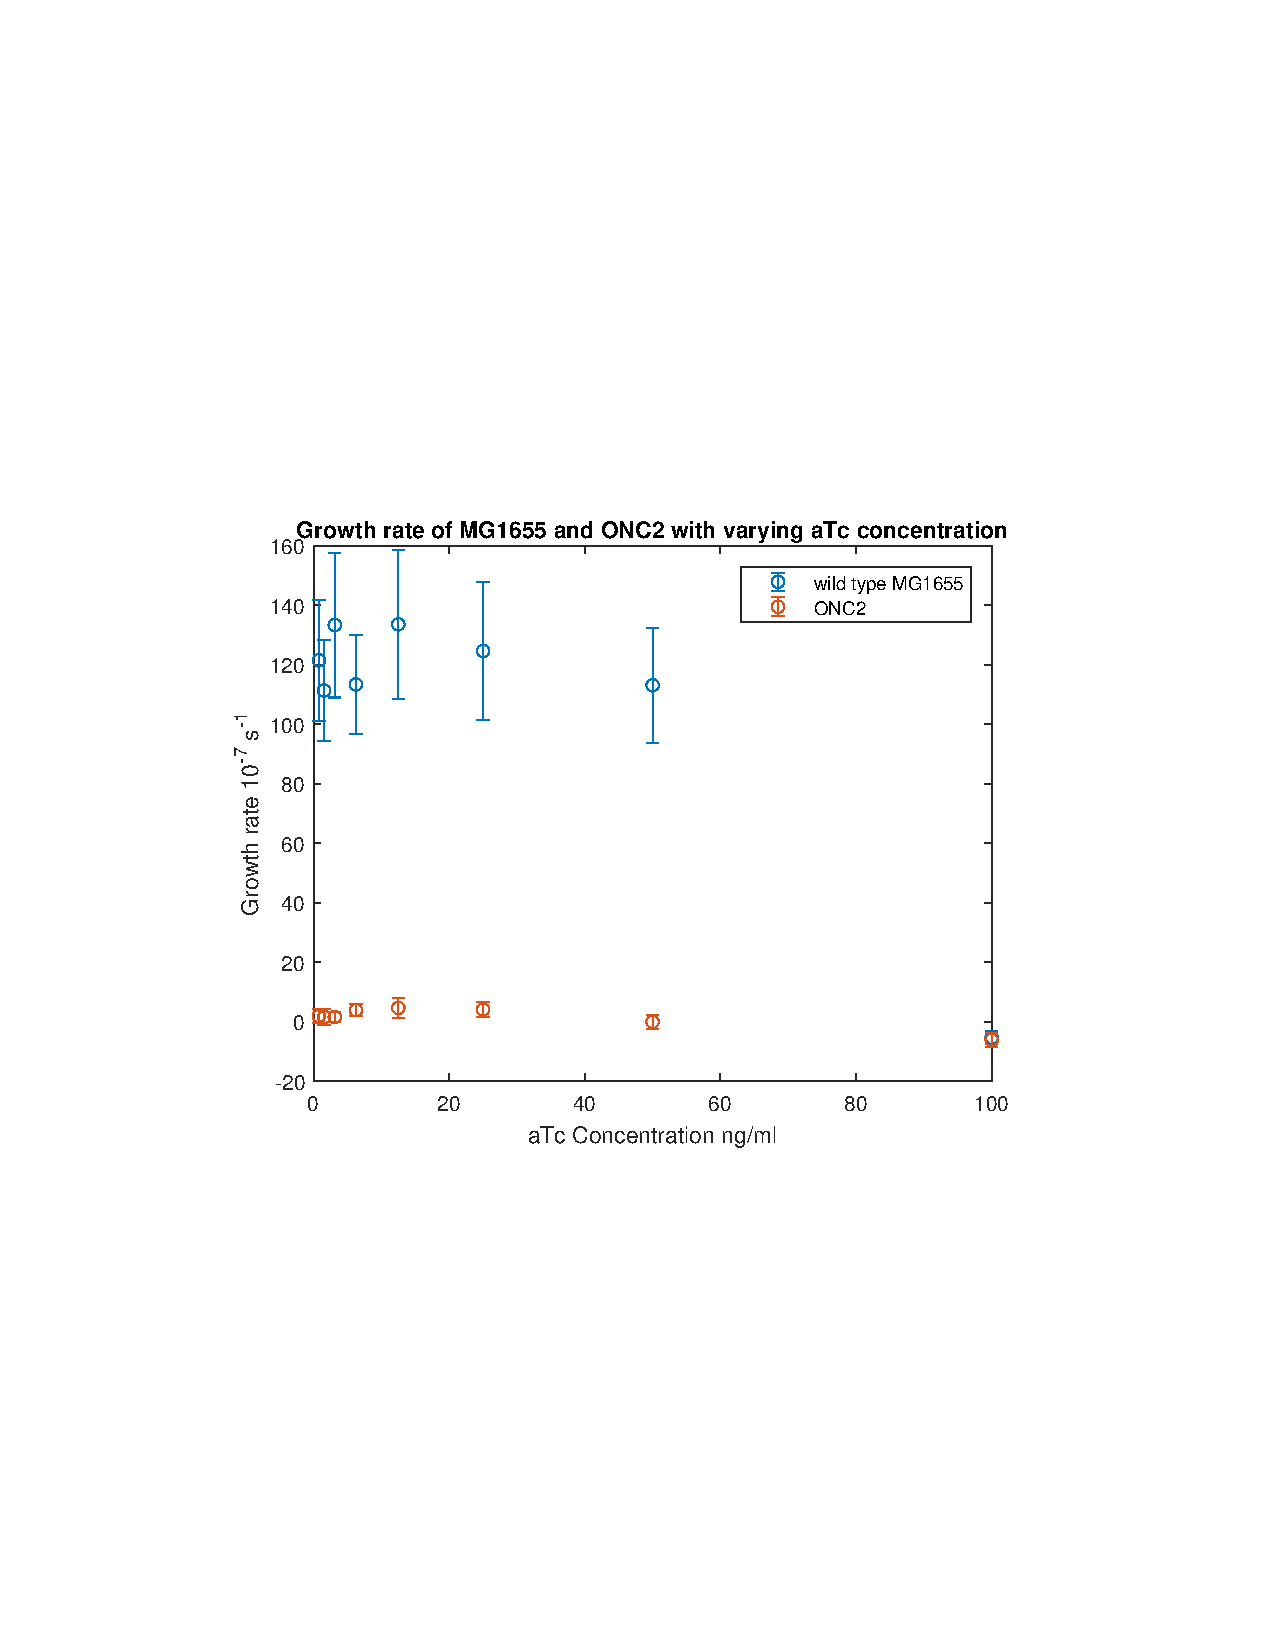
\includegraphics[scale=0.6]{ONC2growthrate.pdf}
\caption{ONC2}
\label{fig:GrowthrateODONC2}
\end{figure}

Figures \ref{fig:GrowthrateODONC1} and \ref{fig:GrowthrateODONC2} represent the plots of growth-rates at different time vs IPTG (or aTc) concentrations. We see that the data for wild type bacteria (denoted in blue) is consistent for the reason mentioned previously, where for the ONC's, it is not satisfactory. 

\section{GFP and RFP intensities and switching rate}
Besides OD, we also measured the fluorescence intensities of the green- and the red- fluorescent proteins (GFP and RFP) in the ONC1 and ONC2 respectively over time. The data for both are not initially comparable. So first we chose background intensities for each ONC's, subtracted them and normalized them by their intensities at initial values (at the beginning of the experiment). Figure \ref{fig:GfpRfpByOD} shows the details about this, where we plotted the GFP/OD and the RFP/OD (denoted green and red respectively) over time. Since OD can be also a good measure for cell-volume, hence GFP/OD and RFP/OD can be interpreted as fluorescence intensities per cell. 

Similar to the OD case, we applied an exponential fit (i.e. a linear fit with logarithmic vertical axis) on the GFP and RFP data and observed the switching rates. 


\begin{figure}[htbp]
\centering
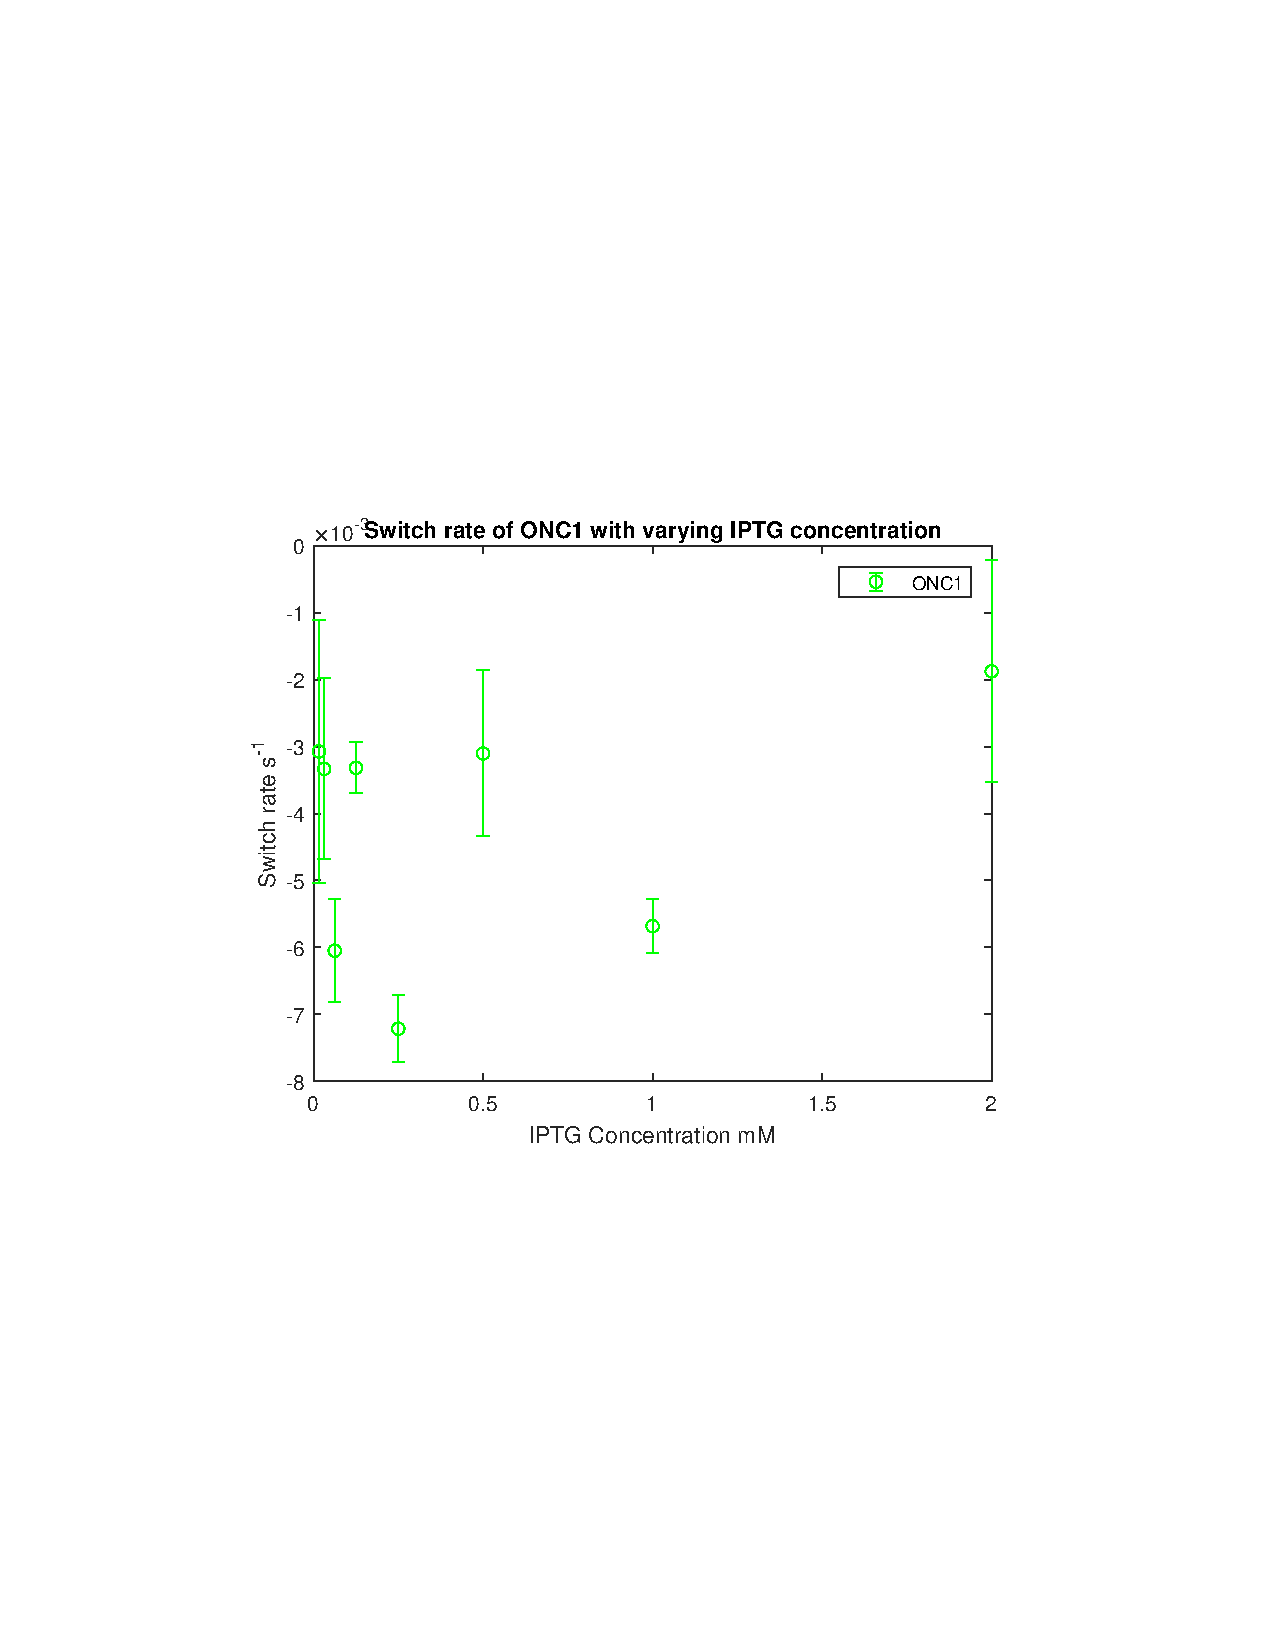
\includegraphics[scale=0.8]{ONC1switchrate.pdf}
\caption{}
\label{fig:onc1SwitchRate}
\end{figure}

\begin{figure}[htbp]
\centering
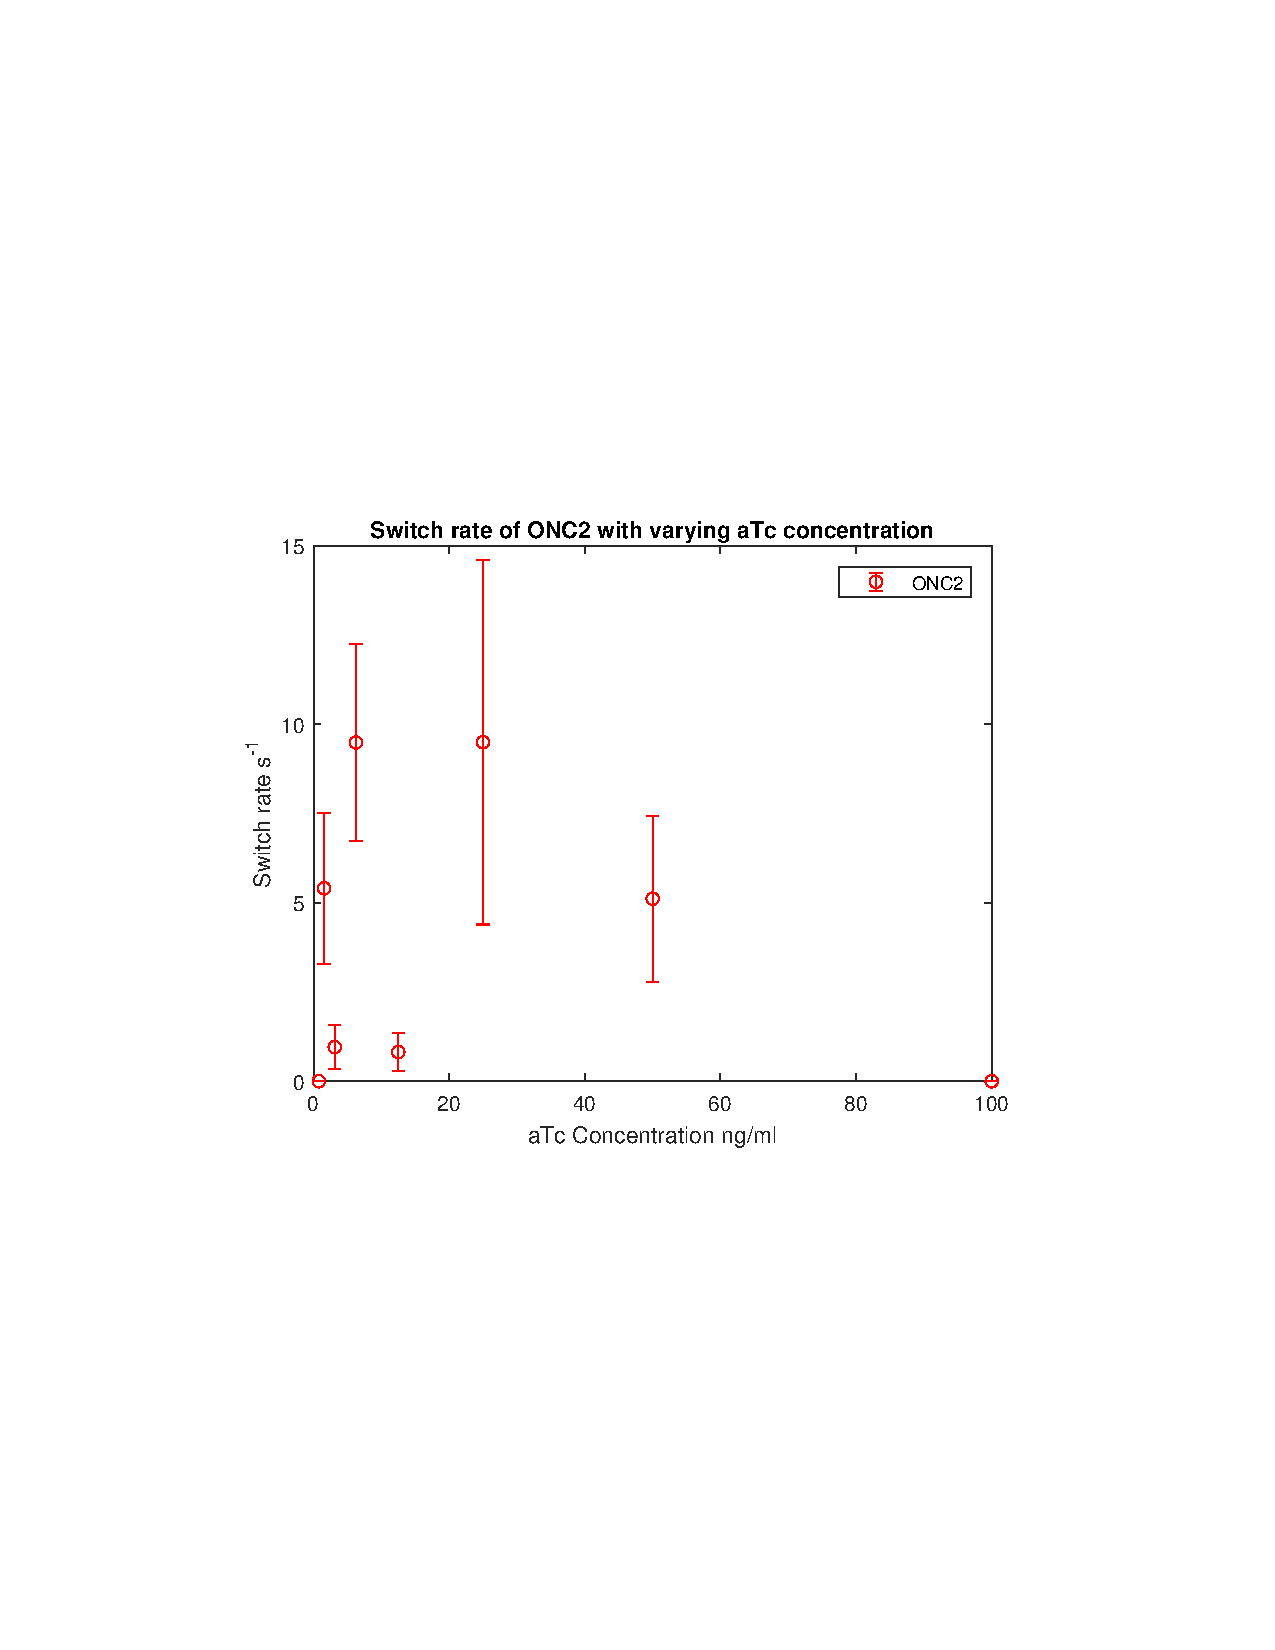
\includegraphics[scale=0.8]{ONC2switchrate.pdf}
\caption{}
\label{fig:onc2SwitchRate}
\end{figure}

Figure \ref{fig:onc1SwitchRate} and \ref{fig:onc2SwitchRate} summarizes the switching rates obtained from the data. Figure \ref{fig:GfpRfpByODLog} shows the background-subtracted and normalized GFP and RFP intensities for each well with a logarithmic vertical axes.

\pagebreak
\section{Single cell fluorescence}
In this part, we took pictures of several bacteria with a microscope and analyzed them. The goal was to observe the switching of the bacterial states by dint of  GFP and RFP intensities. We used \textit{Fiji}, an image processing software to measure the single cell fluorescence of each bacterium in the image. 

\subsection{Composite images}
The following composite images show the green and red fluorescence intensities of ONC1 and ONC2 in different states. 

%--------------green state------------------
\begin{figure}[hbtp]
\centering
	\begin{minipage}{.5\textwidth}
  		\centering
  		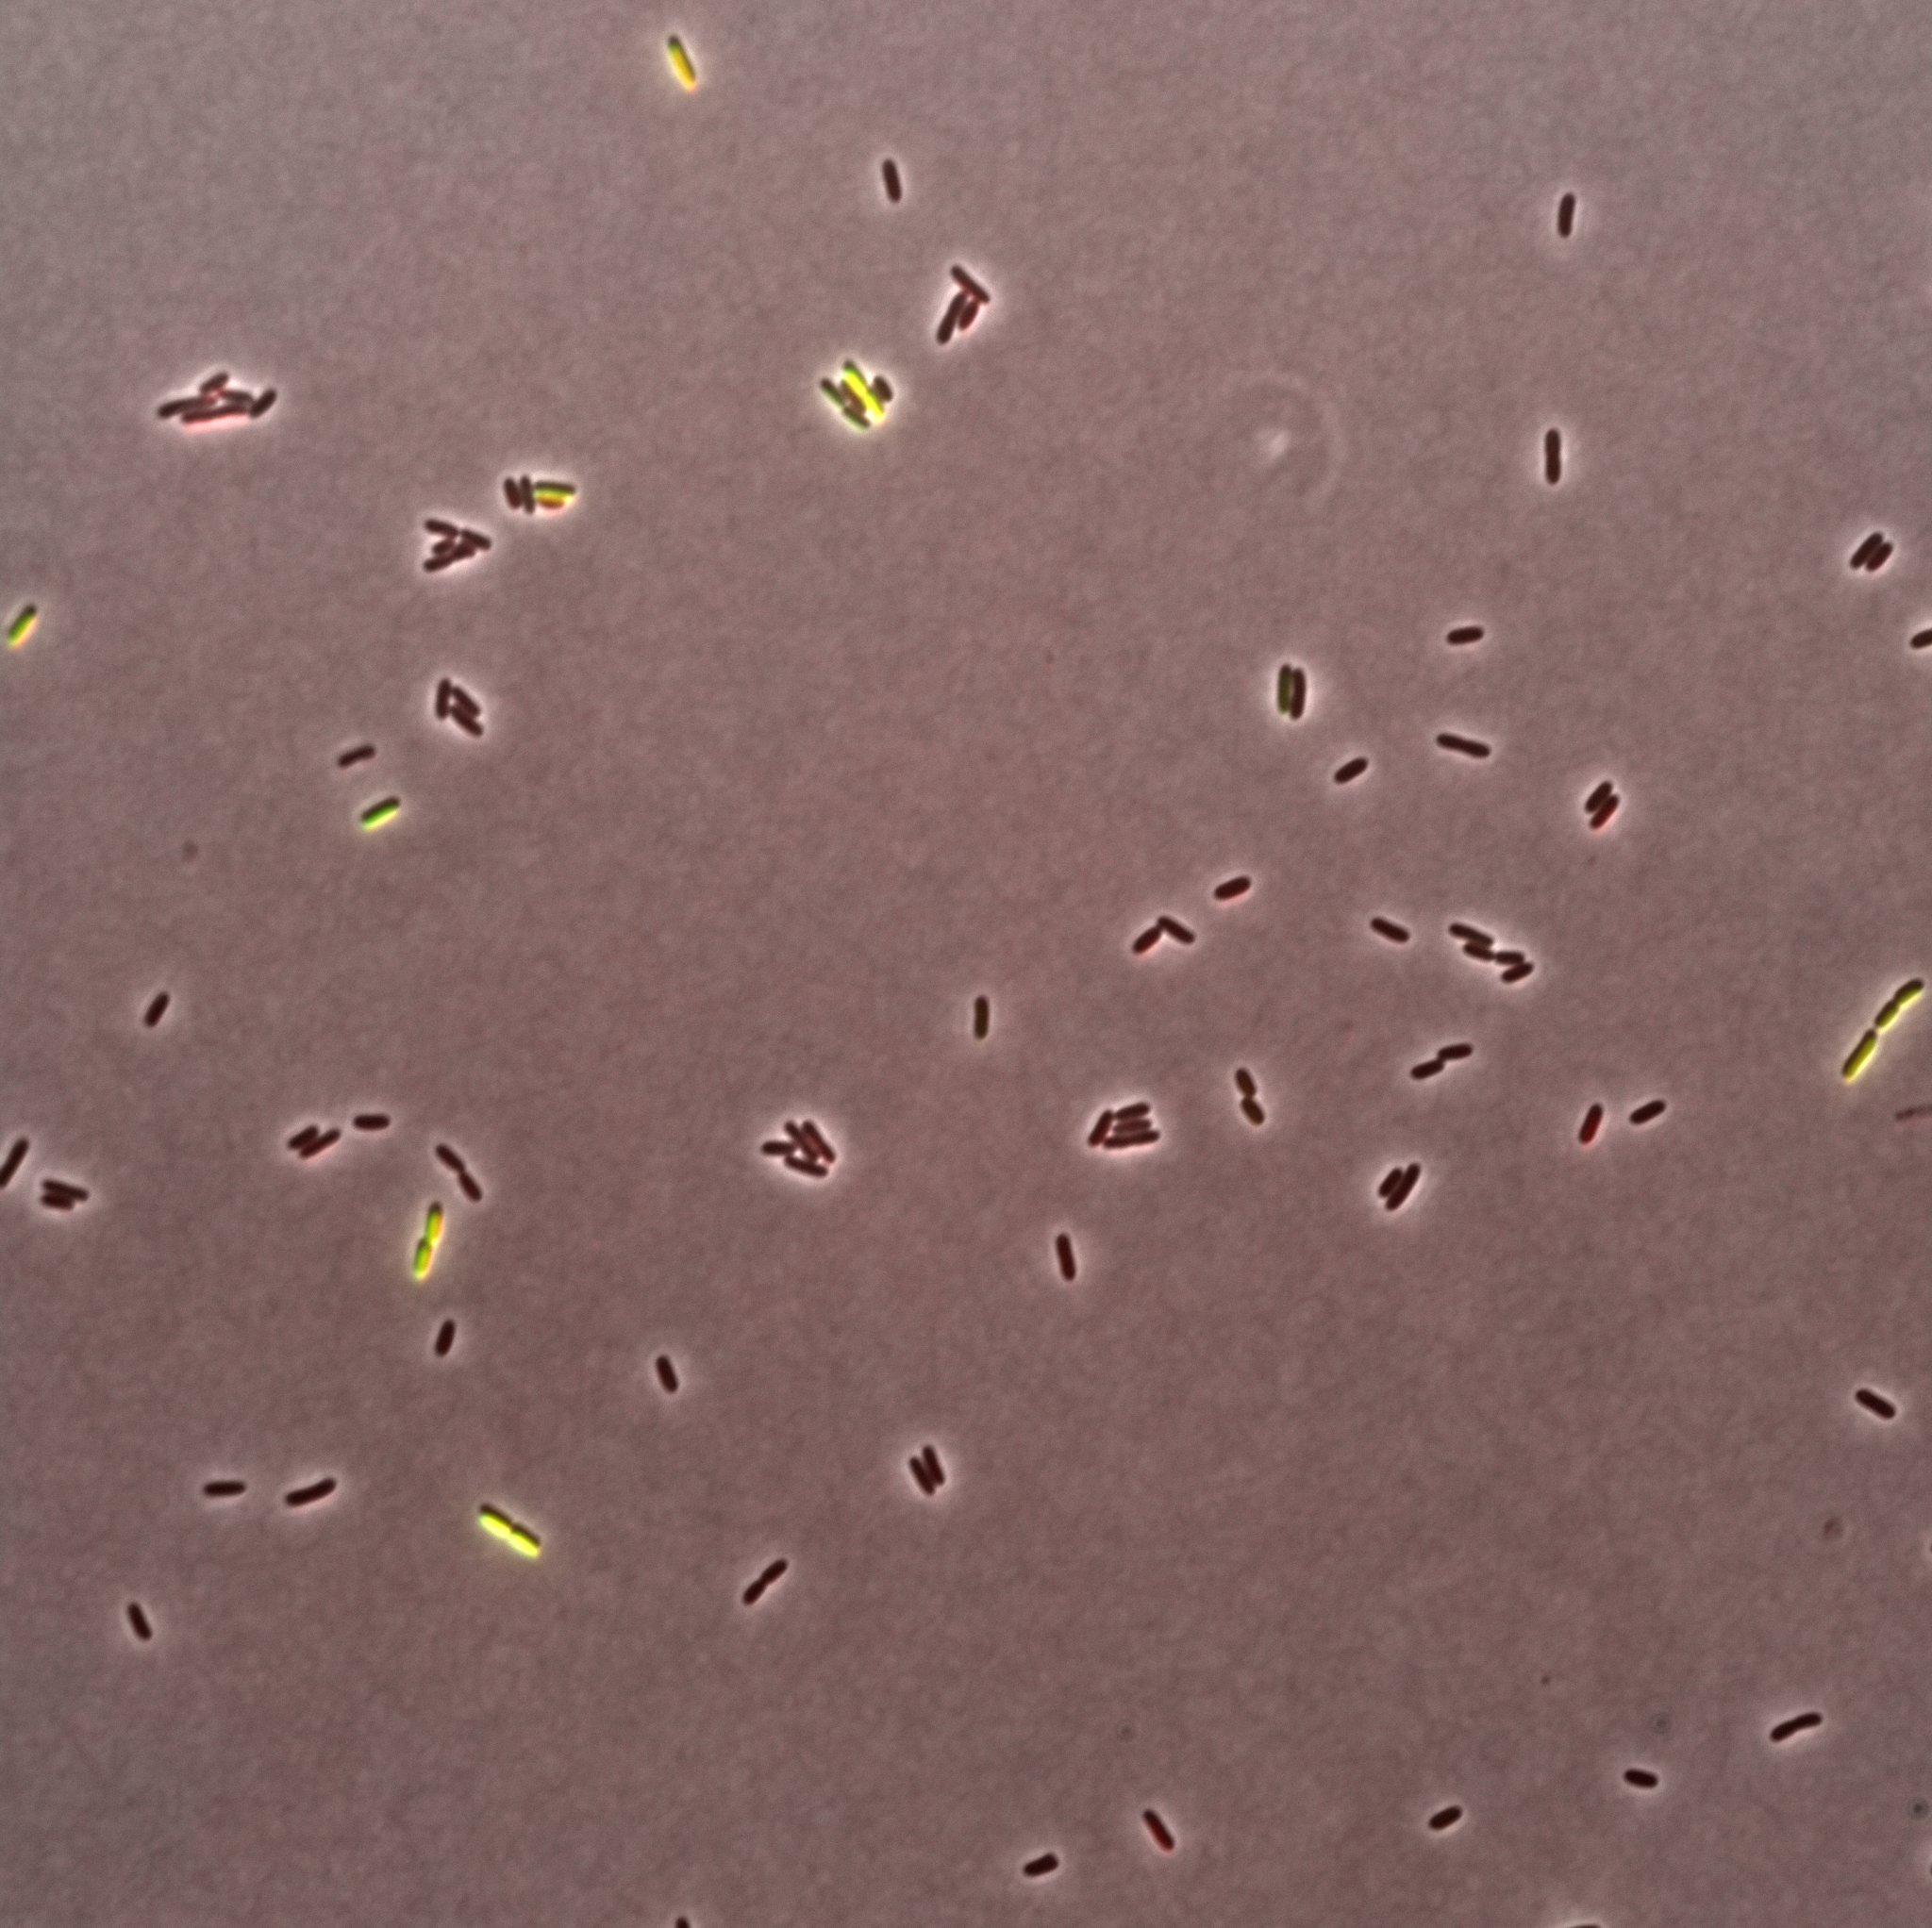
\includegraphics[width=.9\linewidth]{greenstate008Composite.jpg}
  		\captionof{figure}{ONC1 in Green State }
  		\label{fig:onc1GreenStateComposite}
	\end{minipage}%
	\begin{minipage}{.5\textwidth}
  		\centering
  		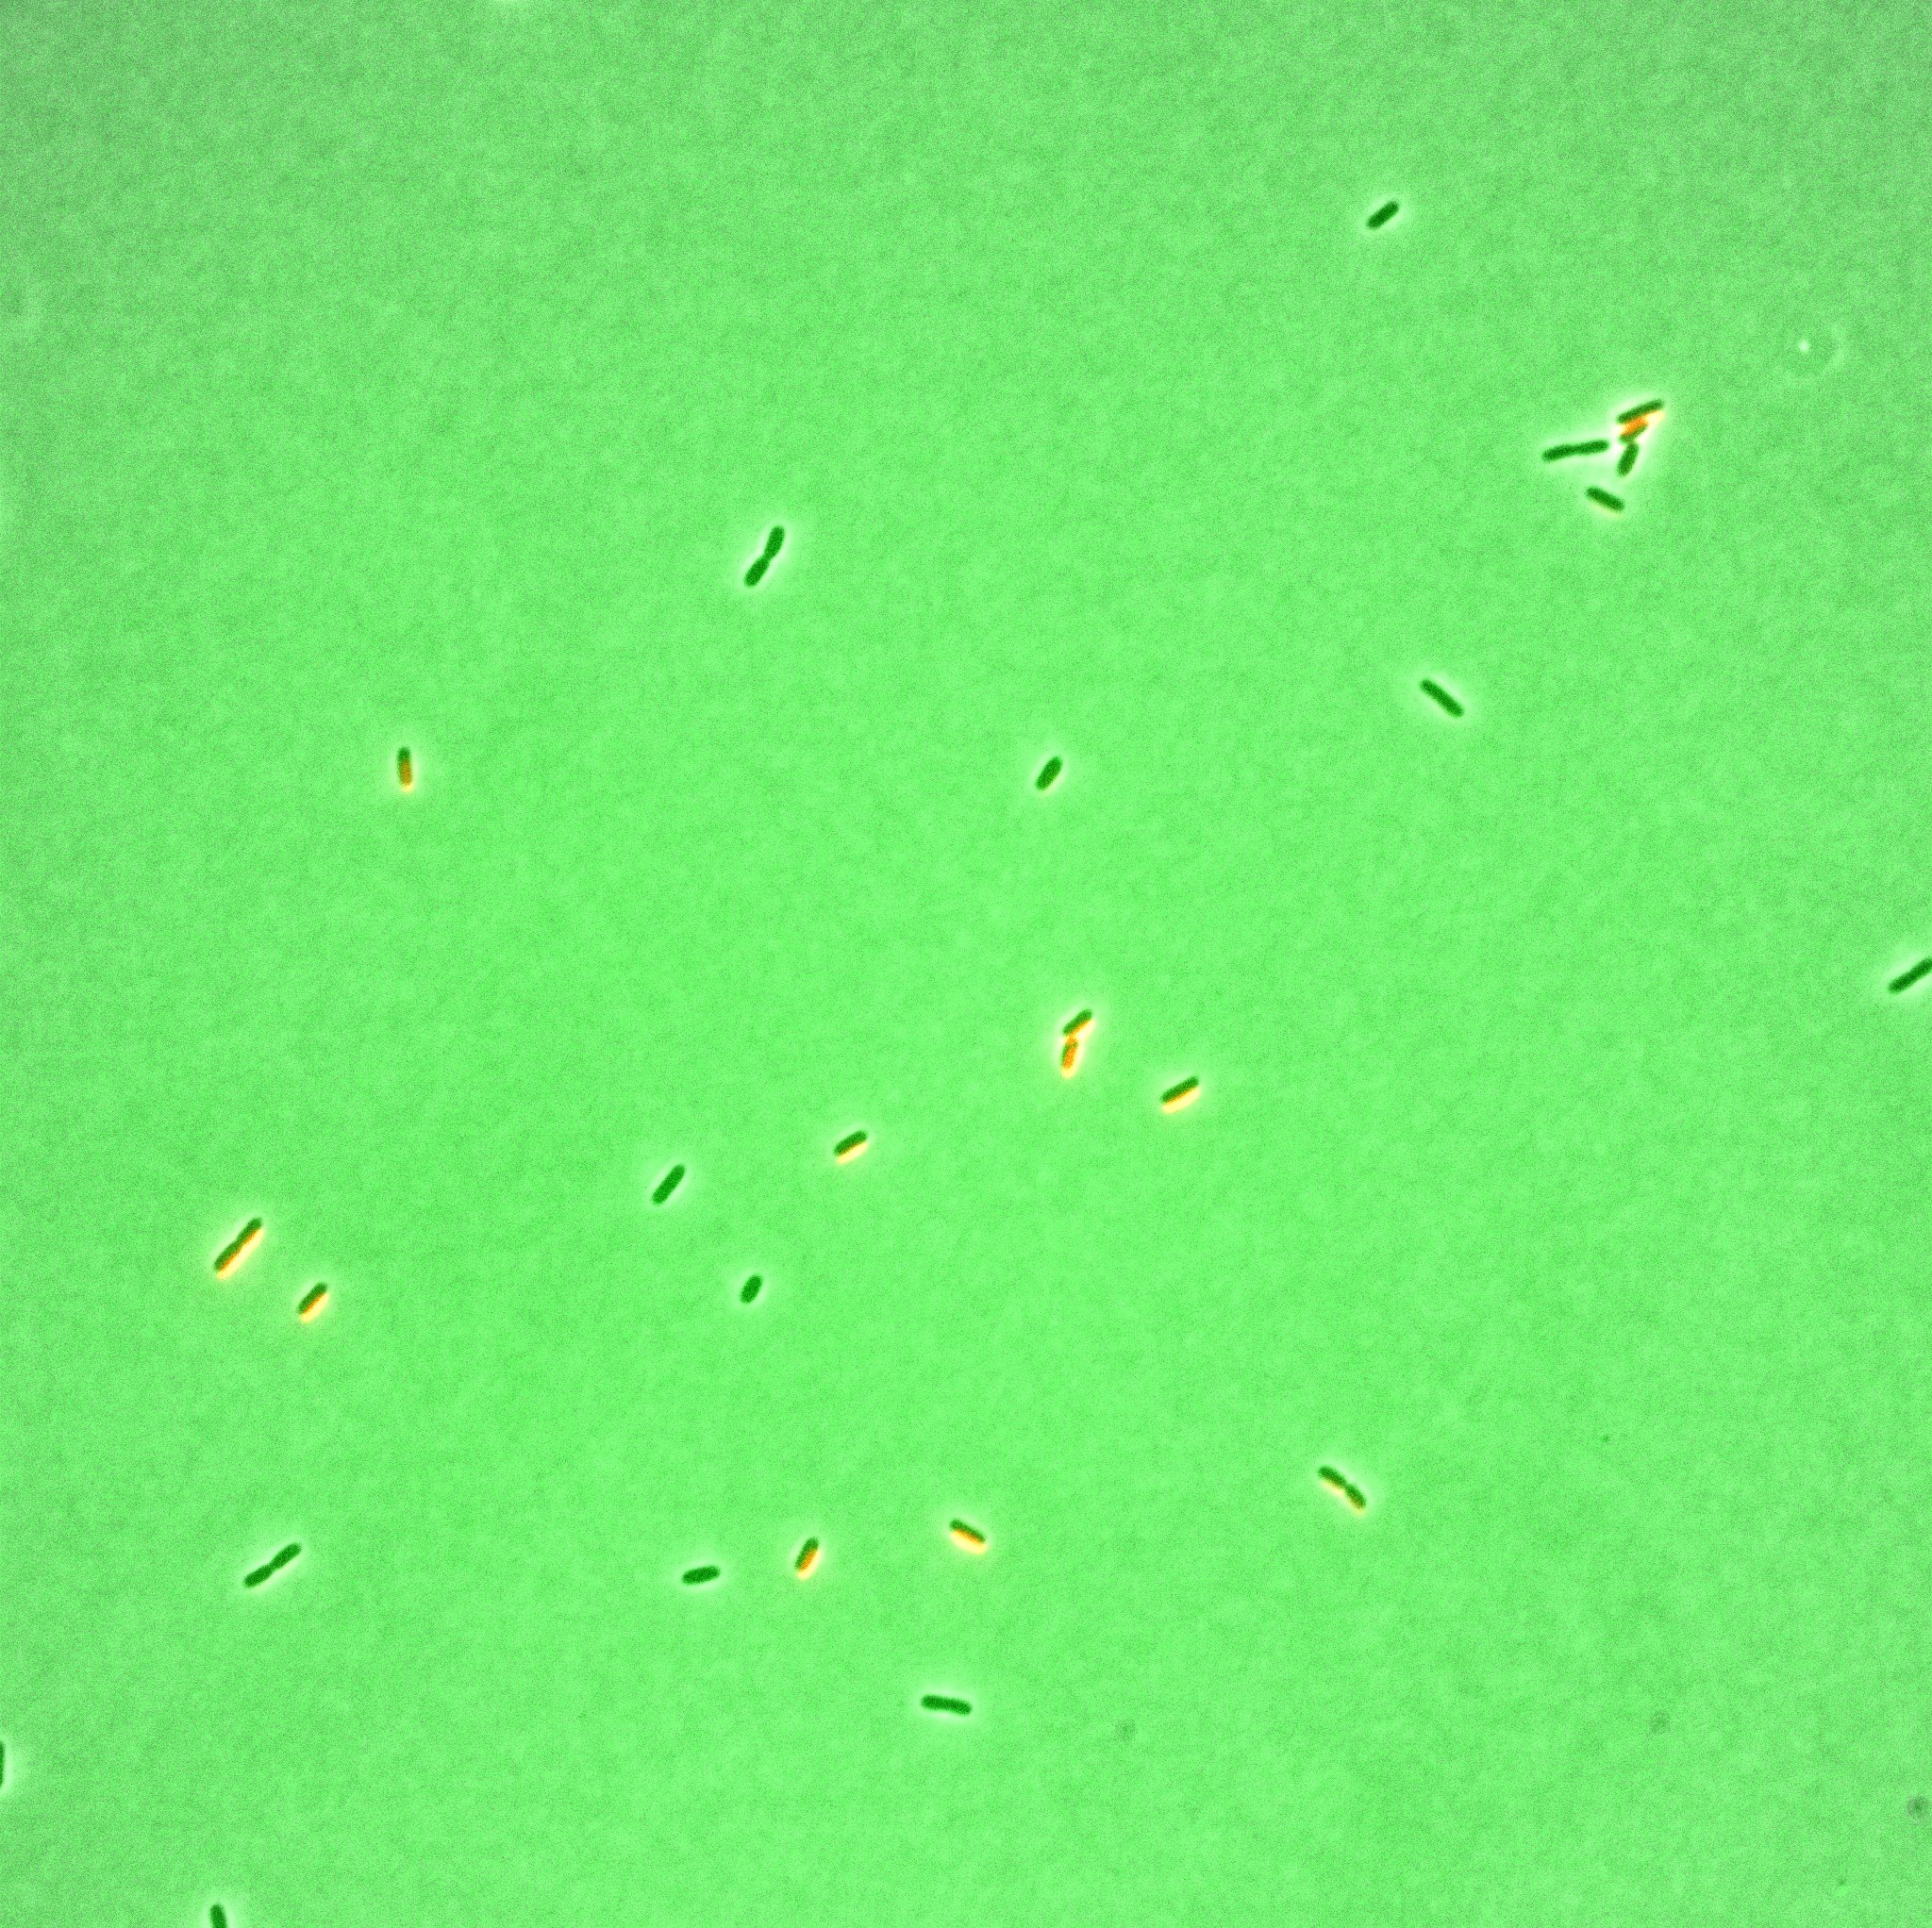
\includegraphics[width=.9\linewidth]{redstate014Composite.jpg}
  		\captionof{figure}{ONC2 in Red State}
  		\label{fig:onc1RedStateComposite}  
	\end{minipage}
\end{figure}

%--------------green state------------------
\begin{figure}[hbtp]
\centering
	\begin{minipage}{.5\textwidth}
  		\centering
  		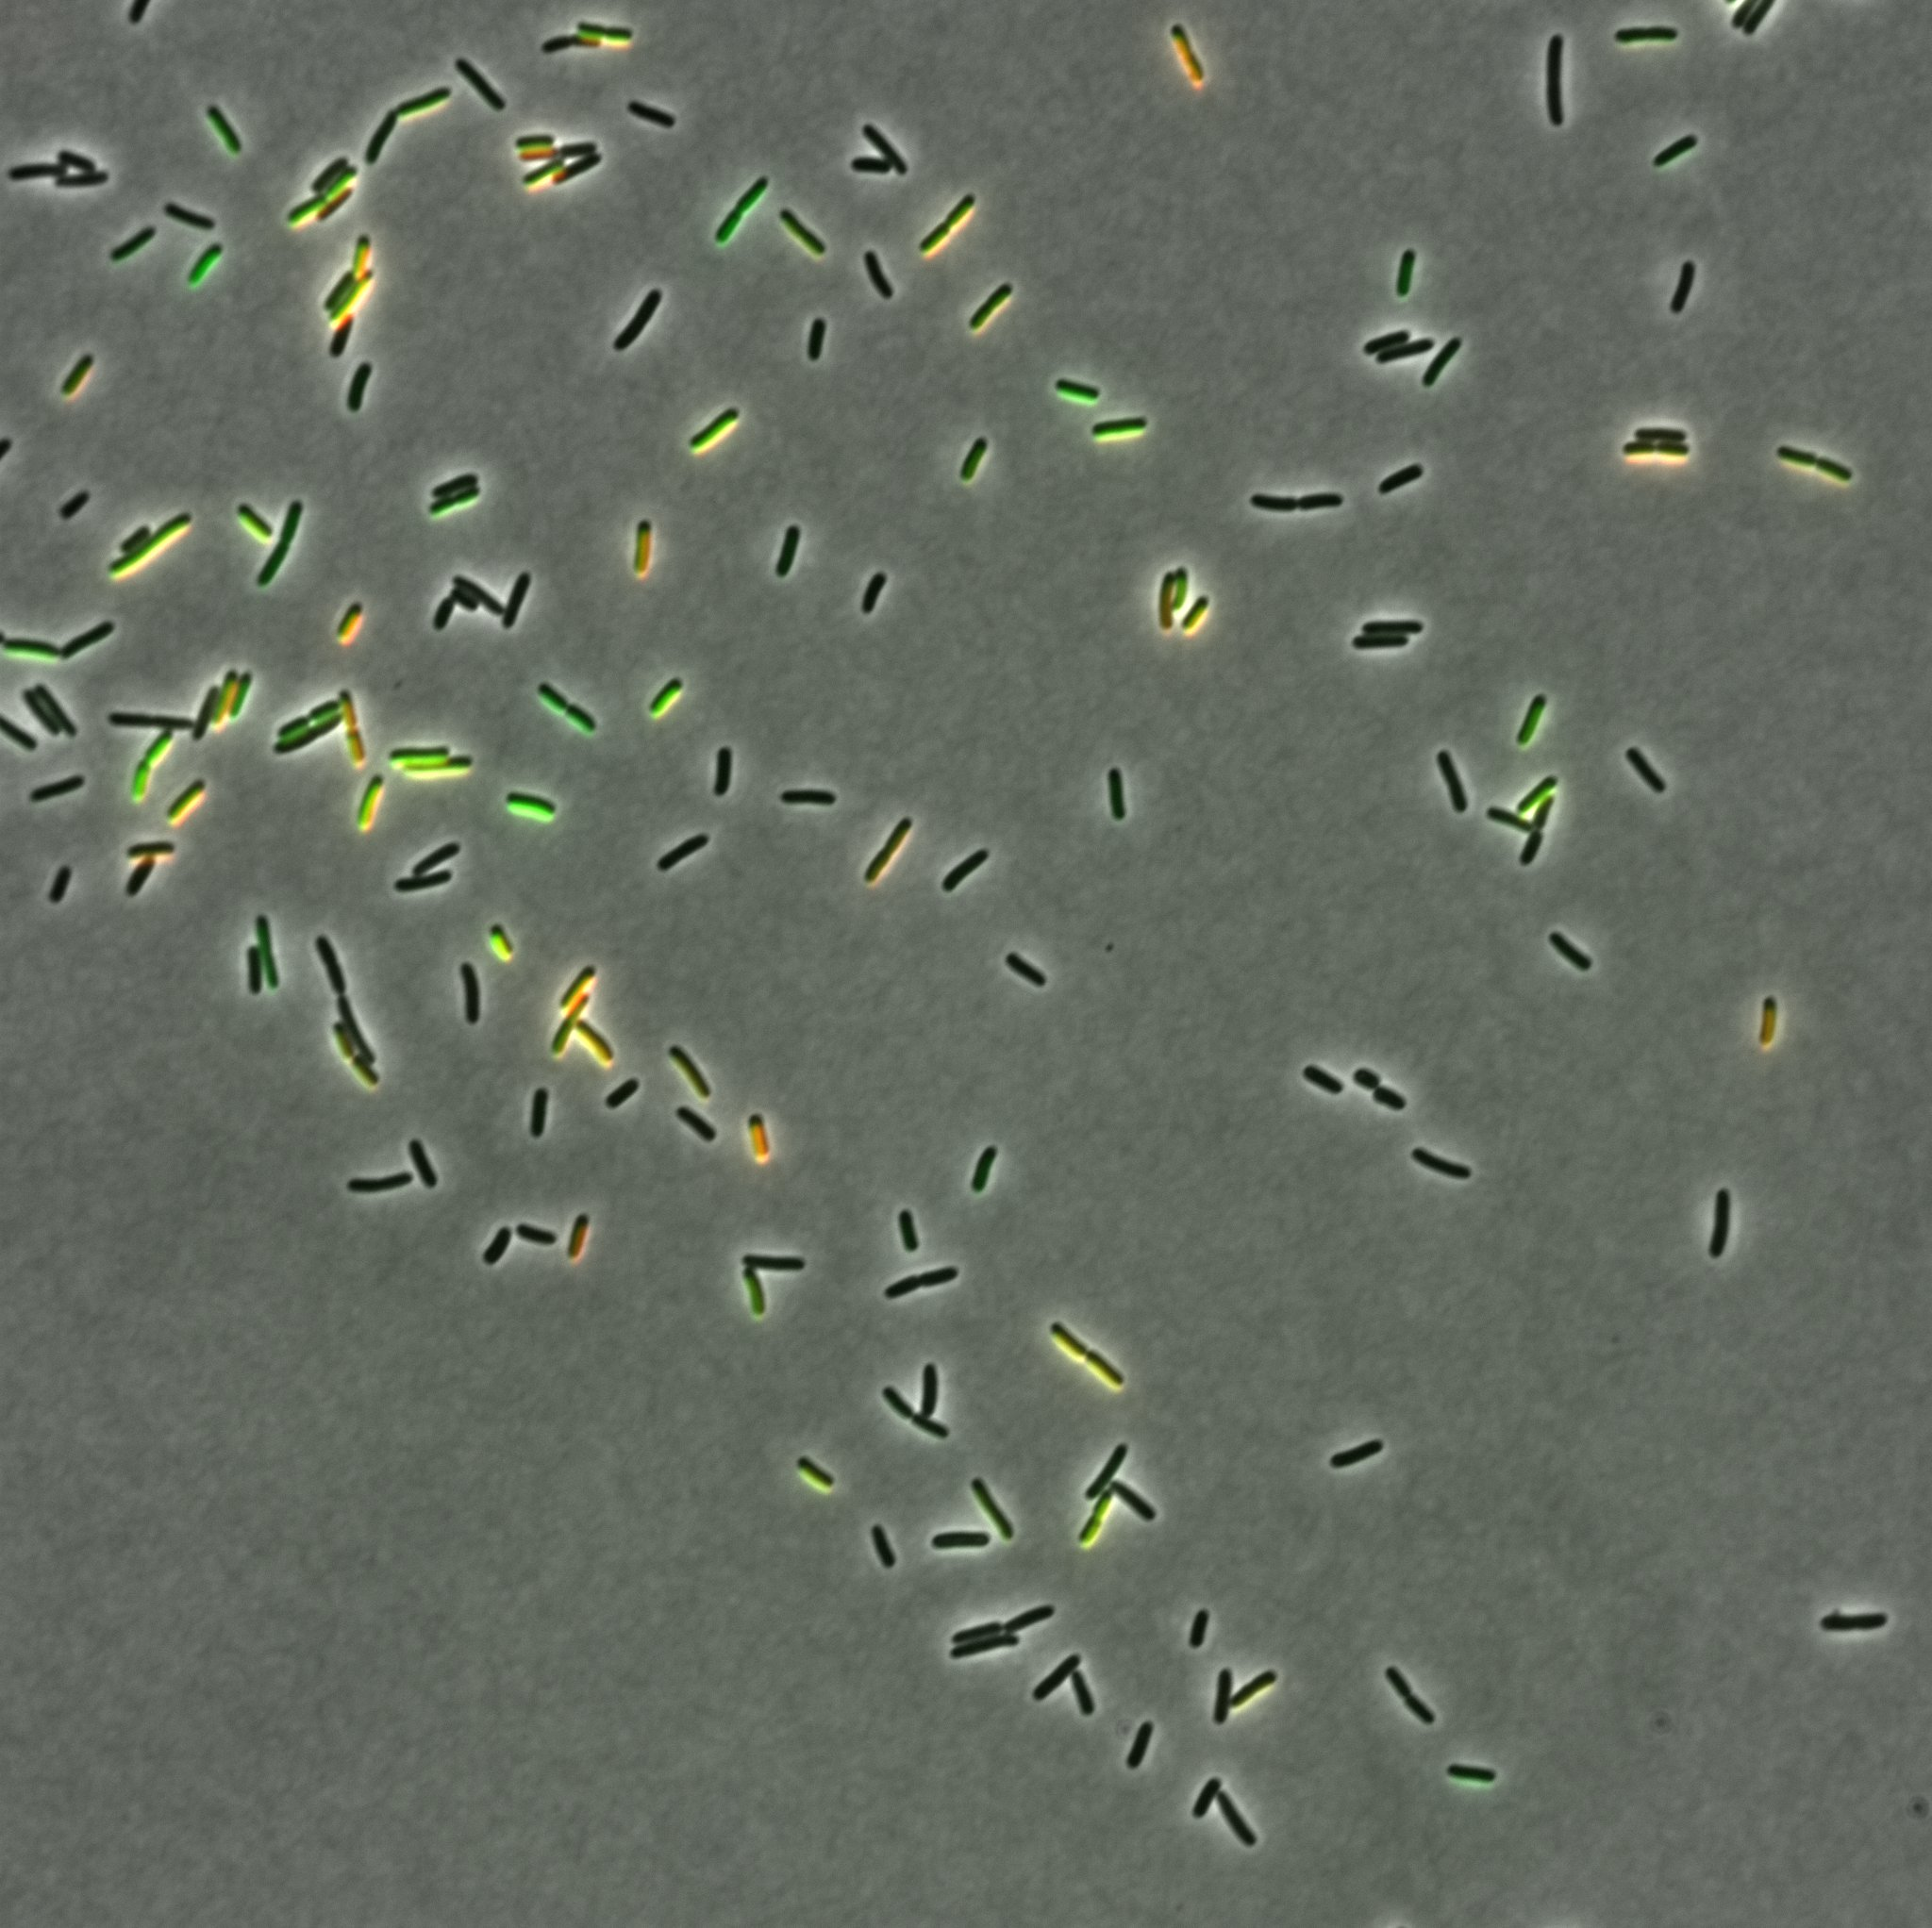
\includegraphics[width=.9\linewidth]{d8007LateComposite.jpg}
  		\captionof{figure}{ONC1 after several hours }
  		\label{fig:onc1AfterHoursComposite}
	\end{minipage}%
	\begin{minipage}{.5\textwidth}
  		\centering
  		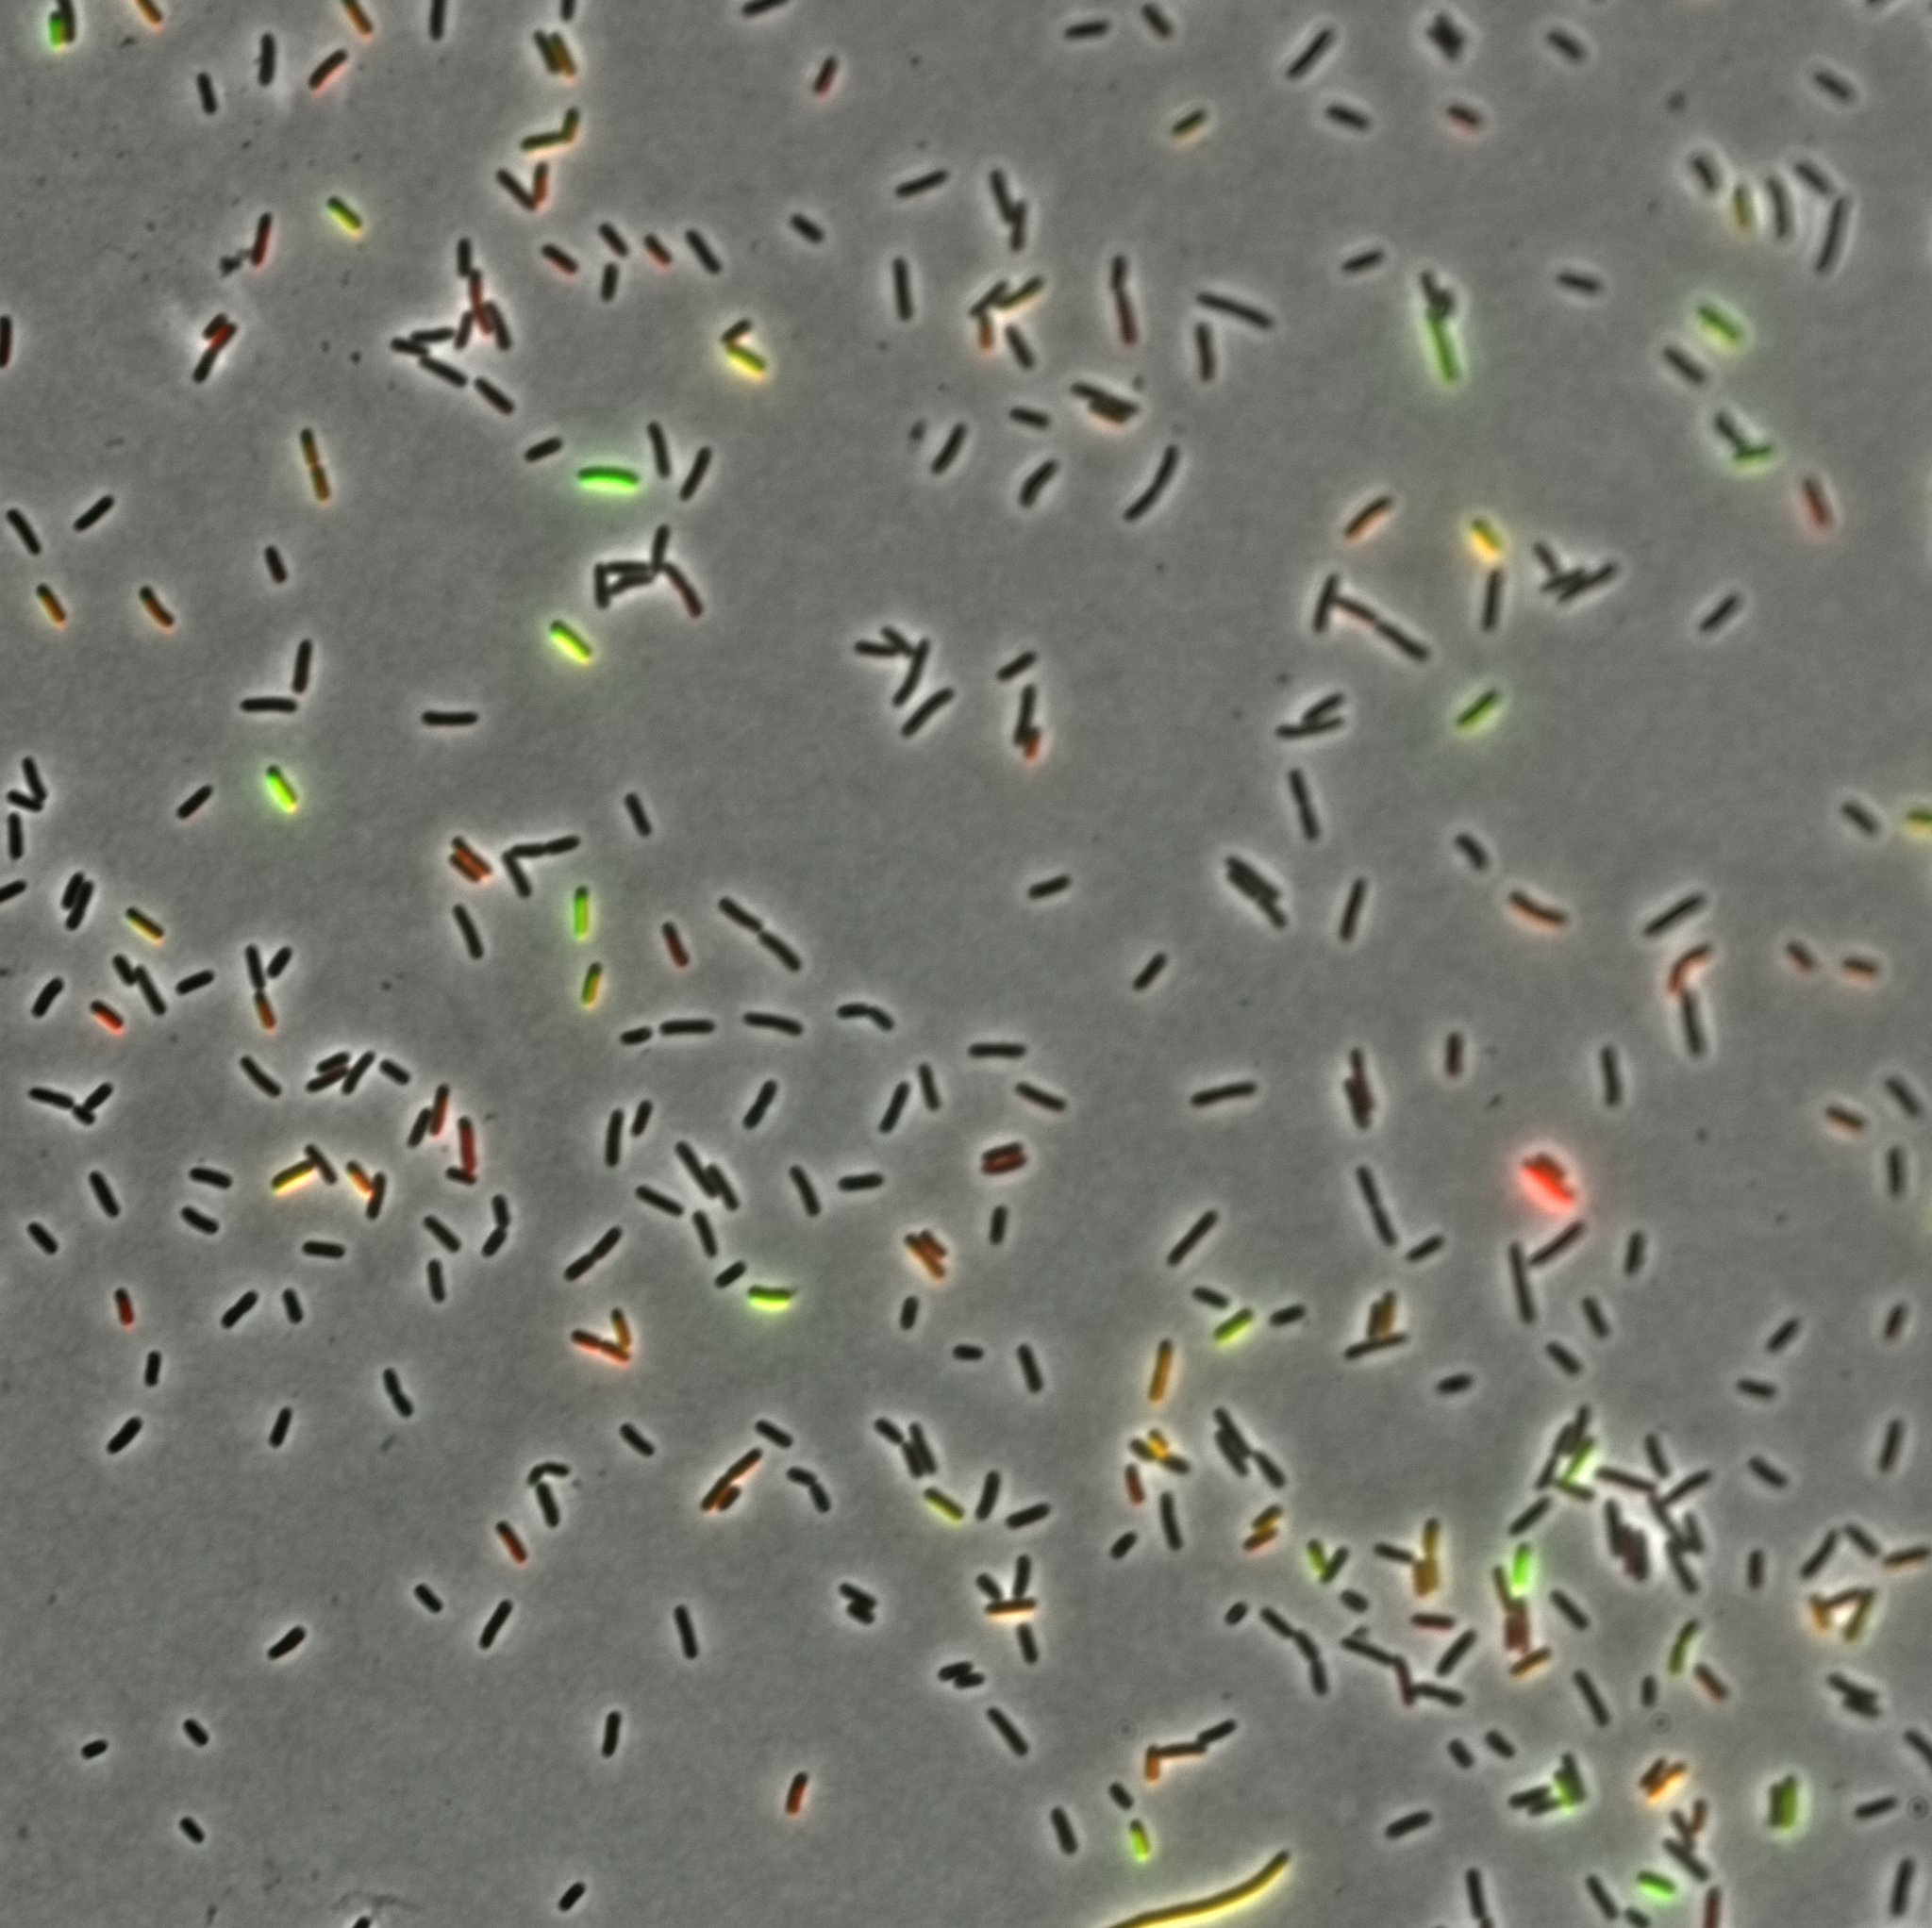
\includegraphics[width=.9\linewidth]{h8LateComposite.jpg}
  		\captionof{figure}{ONC2 after several hours}
  		\label{fig:onc2AfterHoursComposite}  
	\end{minipage}
\end{figure}

At the begining of the experiment, ideally we would expect the ONC1 collection to be completely in green state and the ONC2 in red state. As we can see in the figures \ref{fig:onc1GreenStateComposite} - \ref{fig:onc2AfterHoursComposite}, our samples did not have very strong green and red fluorescence. For the time-evolution, we chose the cultures in the D8 and H8 wells of chart \ref{concGrad}. Both of them were exposed to the highest concentration of IPTG and aTc respectively according to our setup. 

\pagebreak
\subsection{Histograms}
According our image analysis data from Fiji, we quantitatively obtained the green and red fluorescence of the cultures in the images. We generated histograms which indicate a frequency distribution of how many bacteria shine how in which states. 

%--------------green state------------------
\begin{figure}[h]
\centering
	\begin{minipage}{.5\textwidth}
  		\centering
  		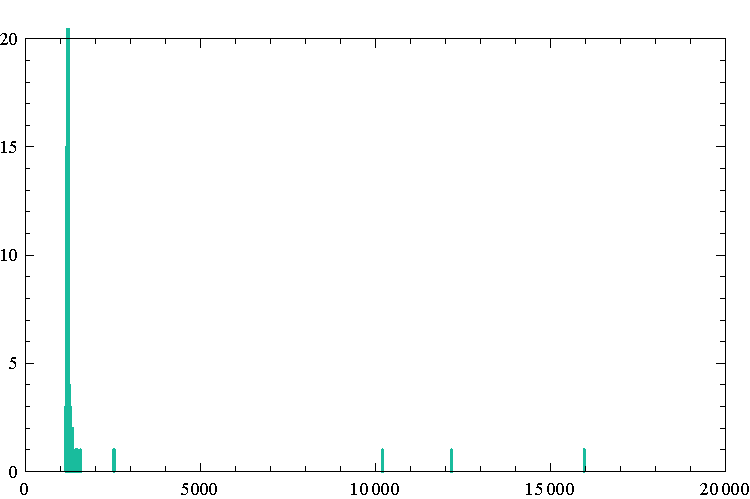
\includegraphics[width=.9\linewidth]{greenstate008GFP.pdf}
  		\captionof{figure}{ONC1 GFP in Green State }
  		\label{fig:onc1GFPGreenState}
	\end{minipage}%
	\begin{minipage}{.5\textwidth}
  		\centering
  		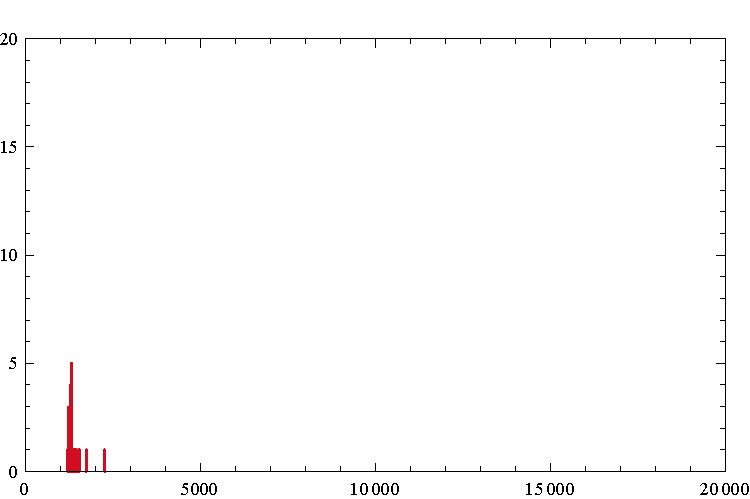
\includegraphics[width=.9\linewidth]{greenstate008RFP.pdf}
  		\captionof{figure}{ONC1 RFP in Green State}
  		\label{fig:onc1RFPGreenState}  
	\end{minipage}
\end{figure}
%--------------red state------------------
\begin{figure}[h]
\centering
	\begin{minipage}{.5\textwidth}
  		\centering
  		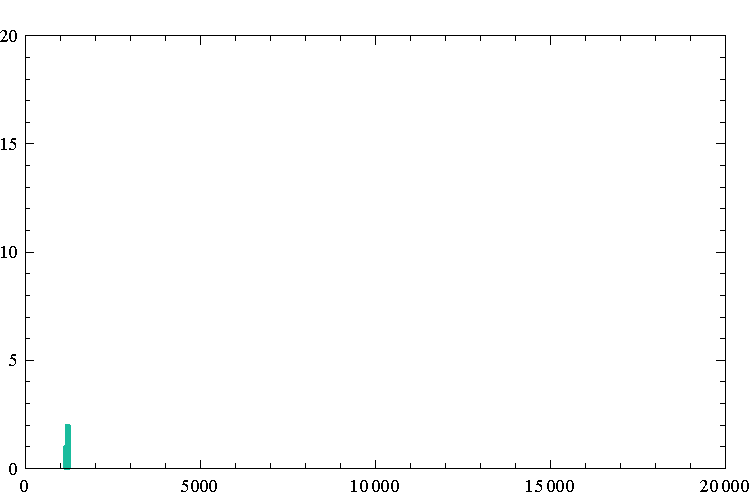
\includegraphics[width=.9\linewidth]{redstate014GFP.pdf}
  		\captionof{figure}{ONC2 GFP in Red State }
  		\label{fig:onc2GFPRedState}
	\end{minipage}%
	\begin{minipage}{.5\textwidth}
  		\centering
  		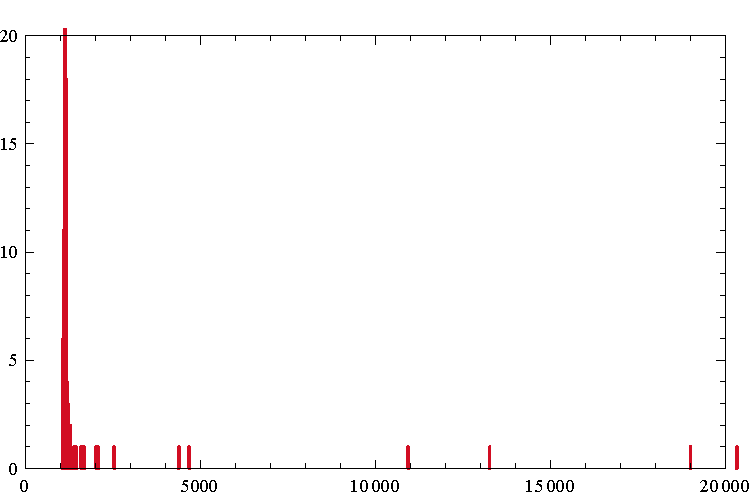
\includegraphics[width=.9\linewidth]{redstate014RFP.pdf}
  		\captionof{figure}{ONC2 RFP in Red State}
  		\label{fig:onc2RFPRedState}  
	\end{minipage}
\end{figure}

%-----green state after time-evolution ------------------
\begin{figure}[h]
\centering
	\begin{minipage}{.5\textwidth}
  		\centering
  		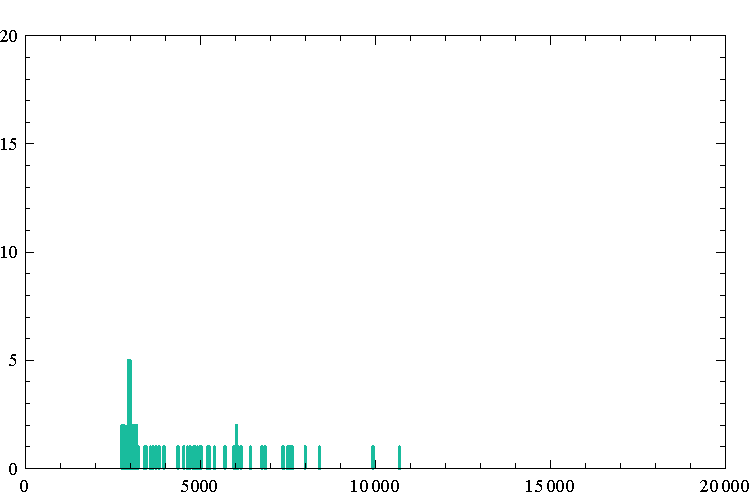
\includegraphics[width=.9\linewidth]{d8007GFP.pdf}
  		\captionof{figure}{ONC1 GFP after several hours }
  		\label{fig:onc1GFPAfterHours}
	\end{minipage}%
	\begin{minipage}{.5\textwidth}
  		\centering
  		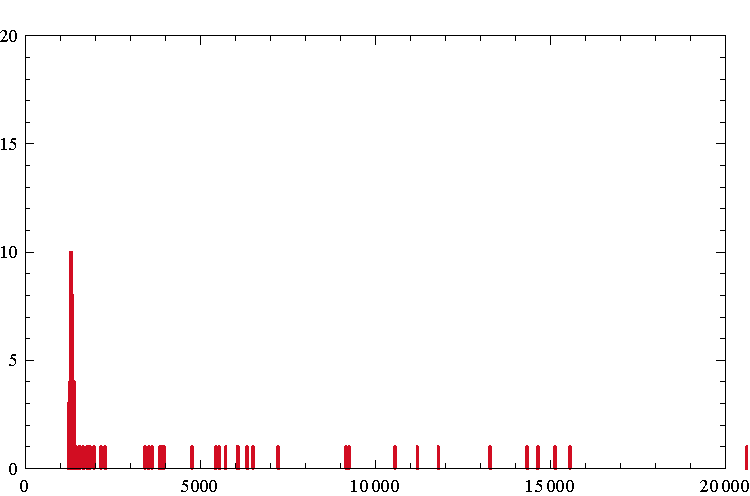
\includegraphics[width=.9\linewidth]{d8007RFP.pdf}
  		\captionof{figure}{ONC1 RFP after several hours}
  		\label{fig:onc1RFPAfterHours}  
	\end{minipage}
\end{figure}

%-----red state after time-evolution ------------------
\begin{figure}[h]
\centering
	\begin{minipage}{.5\textwidth}
  		\centering
  		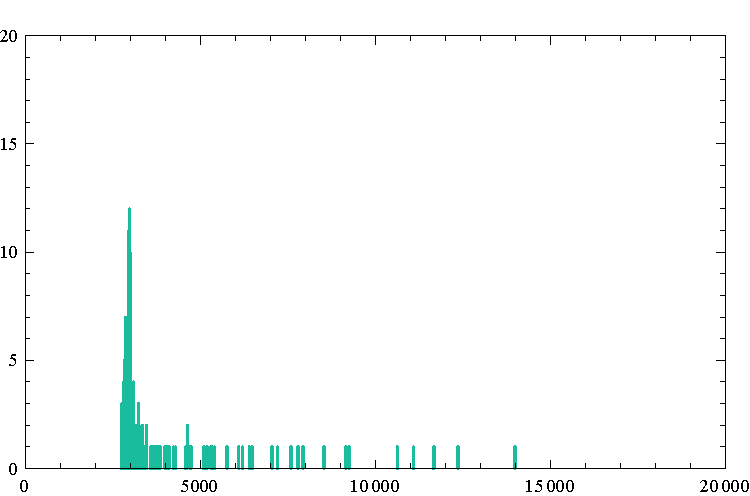
\includegraphics[width=.9\linewidth]{h8LateGFP.pdf}
  		\captionof{figure}{ONC2 GFP after several hours }
  		\label{fig:onc2GFPAfterHours}
	\end{minipage}%
	\begin{minipage}{.5\textwidth}
  		\centering
  		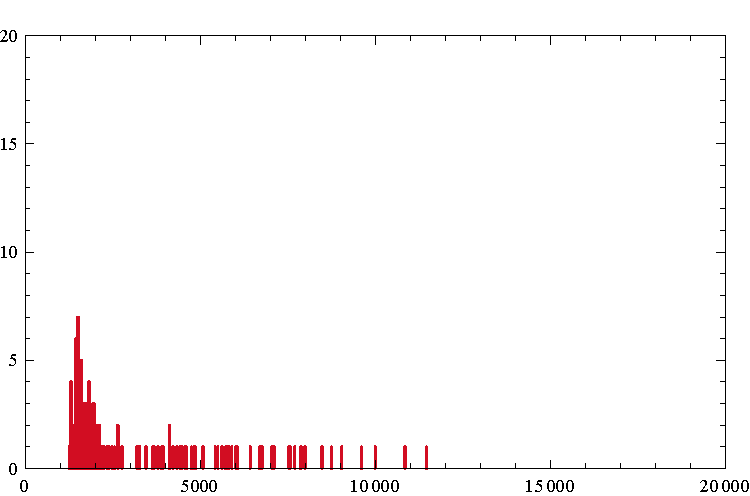
\includegraphics[width=.9\linewidth]{h8LateRFP.pdf}
  		\captionof{figure}{ONC2 RFP after several hours}
  		\label{fig:onc2RFPAfterHours}  
	\end{minipage}
\end{figure}

The first four histograms in the figures \ref{fig:onc1GFPGreenState} - \ref{fig:onc2RFPRedState} show that, most of the  ONC1 bacteria in green state have the high GFP intensity, and ONC2 bacteria have high RFP intensity, as expected. If switching happens, then over a time evolution we would expect the green-state cultures to lose their GFP intensities and red-state cultures to lose their RFP intensities.

The Last four histograms (figures \ref{fig:onc1GFPAfterHours} - \ref{fig:onc2RFPAfterHours}) show that the ONC1 bacteria indeed started losing GFP intensity and gaining the RFP intensity. The opposite happened with the ONC2. So, we can say that the switching started to take place, but was not complete when we reached the end of the experiment. 

\subsection{Switching rate}
Our observation presents the following result

\begin{table}[h]
\centering
\label{switchingRateTable}
\begin{tabular}{lllll}
 	At beginning &  ONC1 &  in Green state	&  97.9730\% $\pm 1\%$ &  \\
	After 4 hrs	 &  ONC1 &  in Green State 	&  61.6279\% $\pm 1\%$ &  \\
	At beginning &  ONC2 &  in Red State	&  92.9134\% $\pm 1\%$ &  \\
	After 4 hrs	 &  ONC2 &  in Red State 	&  80.1762\% $\pm 1\%$ &  \\
\end{tabular}
\caption{Observation of switching}
\end{table}

Hence, approximately $9.1\%$ bacteria switch from Green to Red state in ONC1, and approximately $3.2\%$ bacteria switch from Red to Green state in ONC2. 


\section{Summary}
We have tried to measure the switching between green and red states of the overnight culture of bacteria. We observed that the different concentration do not affect the growth rate of the wild type MG1655 bacteria. For the \textit{E. Coli} bacteria samples, we expected to see the evidence of an increasing growth-rate with IPTG and aTc inducers. From our data of the optical density measurement, it was not very prominent. Also, the GFP and RFP intensity measurements did not present quite promising results. However, direct observation of the microscopic images proved that the switching took place. The green to red switching seemed faster ($9.1\% s^{-1}$) than the red to green switching ($3.2\% s^{-1}$). This might have caused because of the difference in nutrient components or the death of the bacterial cells. 





\begin{thebibliography}{999}
	\bibitem{labManual}
	Laboratory Manual on Genetic Toggle Switch Experiment, Biophysics Practical course, University of Cologne
	\bibitem{gitRepo}
    	\url{https://github.com/galibhassan/Genetic-Toggle-Switch-Lab}
\end{thebibliography}







\pagebreak
\part{Appendix}



\begin{figure}[h]
\centering
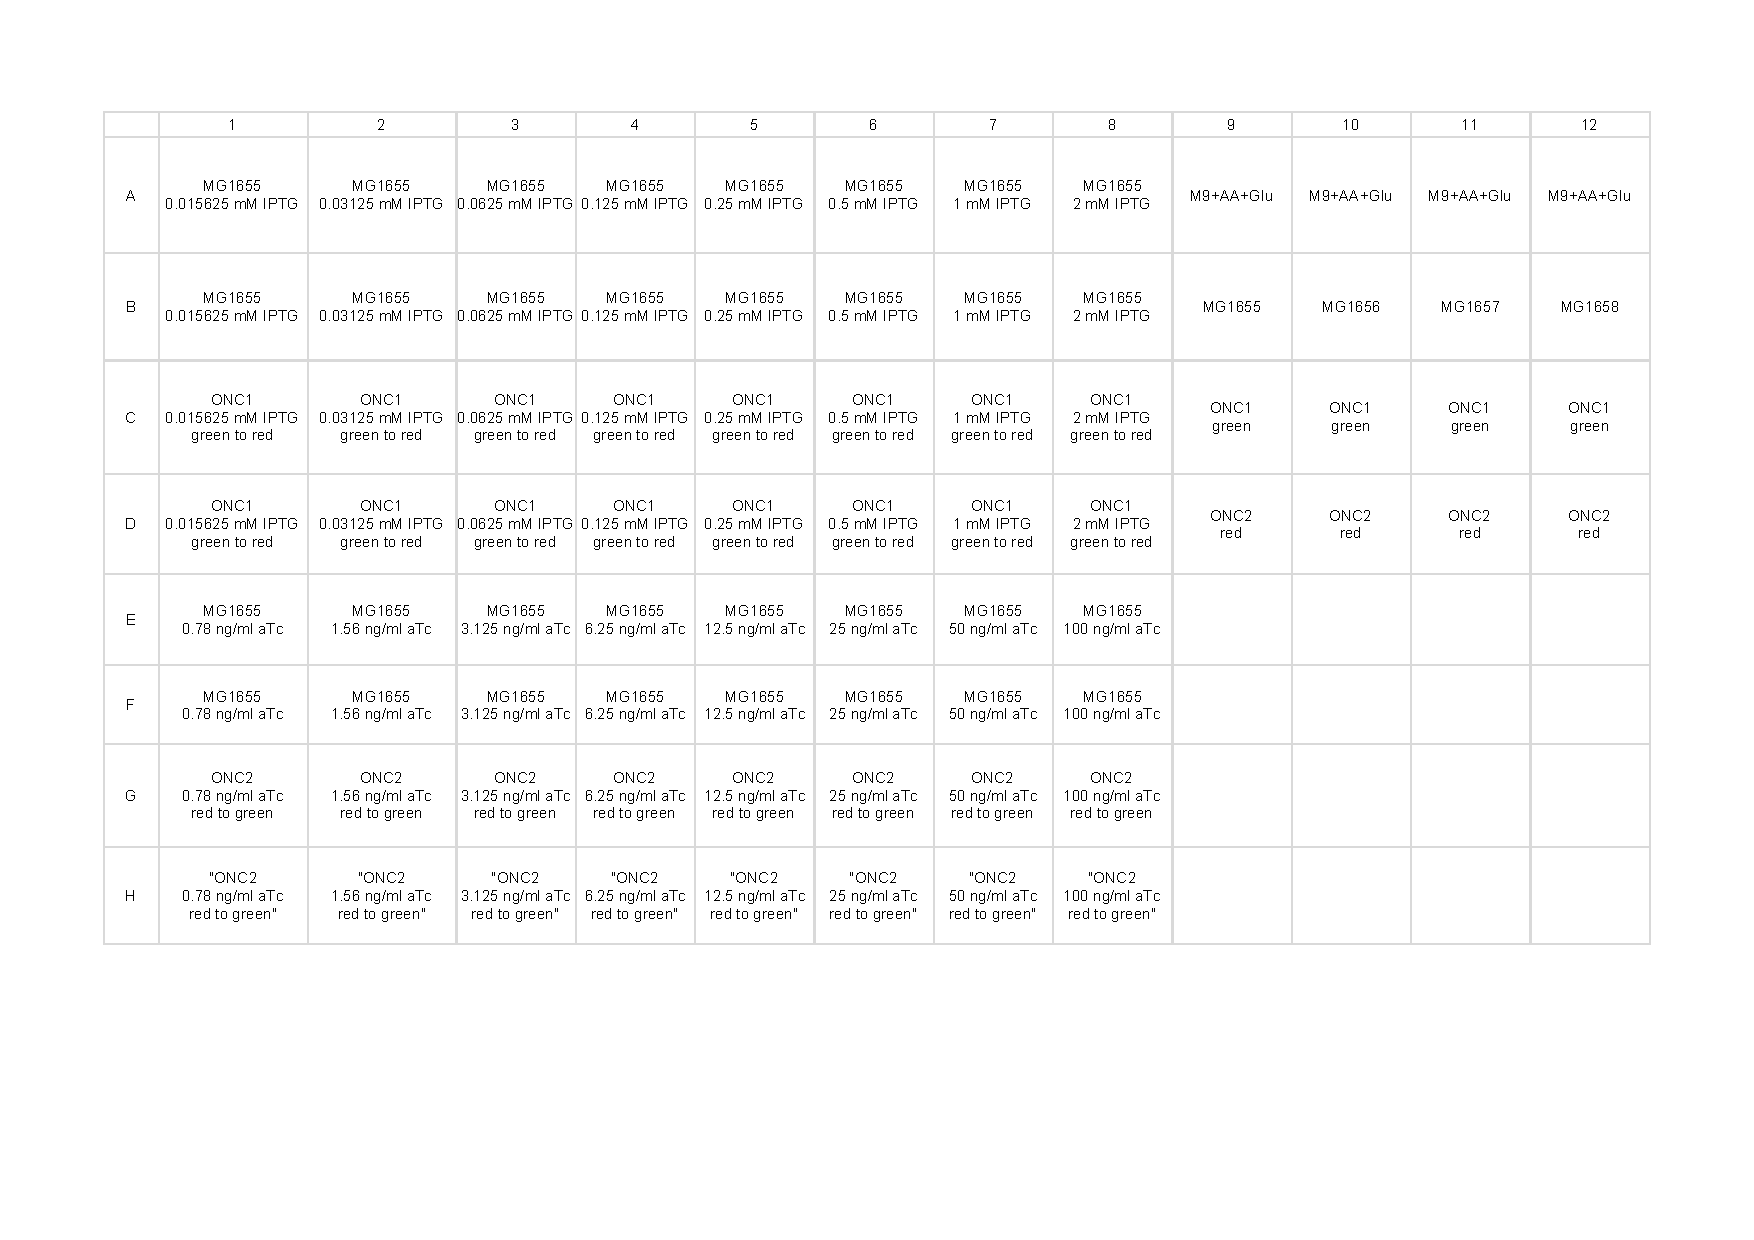
\includegraphics[scale=0.7, angle=-90, origin=c]{concentrationGradient}
\caption{Concentration gradient of IPTG and aTc}
\label{concGrad}
\end{figure}

\pagebreak

\begin{figure}[htbp]
\centering
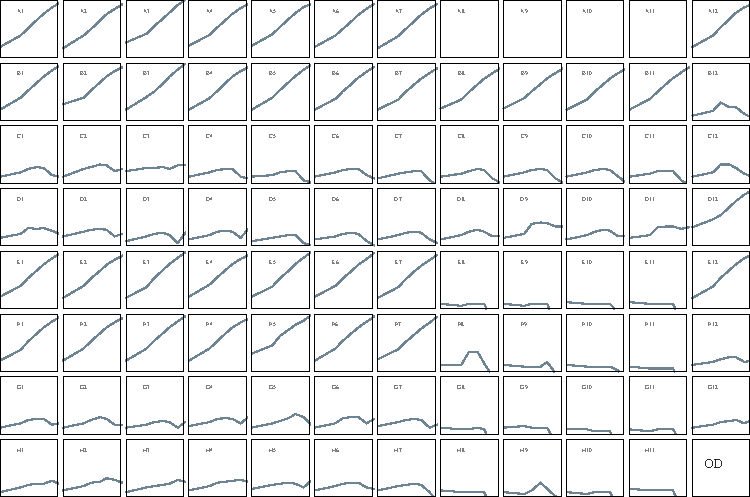
\includegraphics[scale=1.5, angle=-90, origin=c]{OD-LogPlot.pdf}
\caption{
Optical Density of each well in figure \ref{concGrad} (measured over time from 0 to 14000 seconds in horizontal axes). The Vertical axes are logarithmic.}
\label{ODLogPlot}
\end{figure}


\begin{figure}[h]
\centering
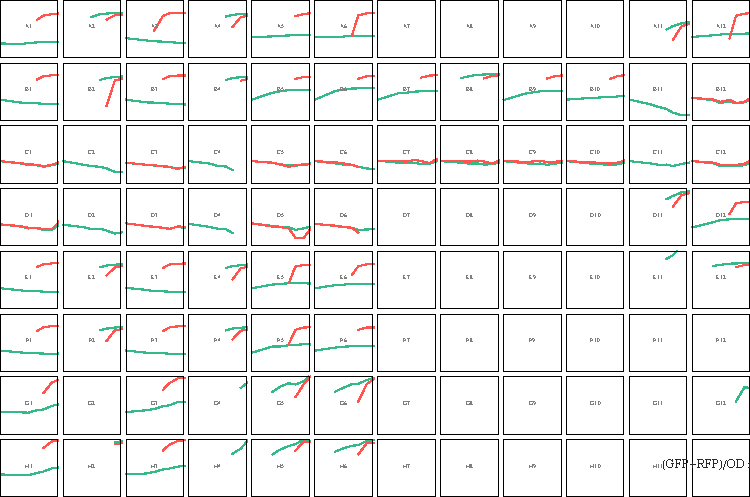
\includegraphics[scale=1.5, angle=-90, origin=c]{LogGfpPlusRfpByODCorrectedYMax12.pdf}
\caption{Background corrected and normalized GFP/OD and RFP/OD over time. The Vertical axes are logarithmic.}	
\label{fig:GfpRfpByODLog}
\end{figure}





\end{document}

